\documentclass{beamer}
\usepackage[utf8]{inputenc}
\usepackage{amsfonts} %math support

\beamertemplatenavigationsymbolsempty %removes navigation bar

\usepackage{tcolorbox}%for colored boxes
\usepackage{stix}%male female symbiols

%\defbeamertemplate{footline}{centered page number}
%{%
%  \hspace*{\fill}%
%  \usebeamercolor[fg]{page number in head/foot}%
%  \usebeamerfont{page number in head/foot}%
%  Scott, \textbf{Osmond}, Otto%
%  \hspace*{\fill}\vskip2pt%
%}
%\setbeamertemplate{footline}[centered page number]

\defbeamertemplate{headline}{centered page number}
{%
  \vspace{0.1cm}
  \hspace*{\fill}%
  \usebeamercolor[fg]{page number in head/foot}%
  \usebeamerfont{page number in head/foot}%
  Scott, \textbf{Osmond}, Otto [\insertframenumber\,/\,\inserttotalframenumber] \hspace{0.1cm}%
%  \hspace*{\fill}
%  \vskip2pt%
}
\setbeamertemplate{headline}[centered page number]

\usepackage{tikz}
\usetikzlibrary{calc}
\usetikzlibrary{decorations.pathreplacing}
\def\checkmark{\tikz\fill[scale=1](0,.35) -- (.25,0) -- (1,.7) -- (.25,.15) -- cycle;} 

\title{Gametic selection, meiotic drive, sex ratio bias, and transitions b/w sex determination systems}
\author{Matthew Osmond$^2$}
\institute{$^1$University College London \& $^2$University of British Columbia}
\date{Evolution 2017}
\titlegraphic{\vspace{3cm}} %lifts text up

\begin{document}

%%%%%%%%%%%%%%%%%%%%%%%%%%%%%%%%%%%%%%%%%%%%%%%%%
%%\frame{\titlepage}
%\begin{frame}[plain]
%   \begin{tikzpicture}[overlay, remember picture]
%      \node[anchor = south east] at (current page.south east) {
%         \scalebox{-1}[1]{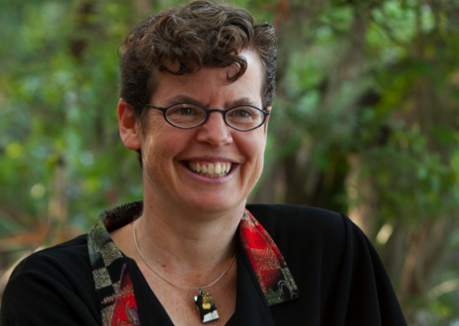
\includegraphics[width=0.5\textwidth]{IMAGES/Sally}}
%      };
%      \node[anchor = south west] at (current page.south west) {
%         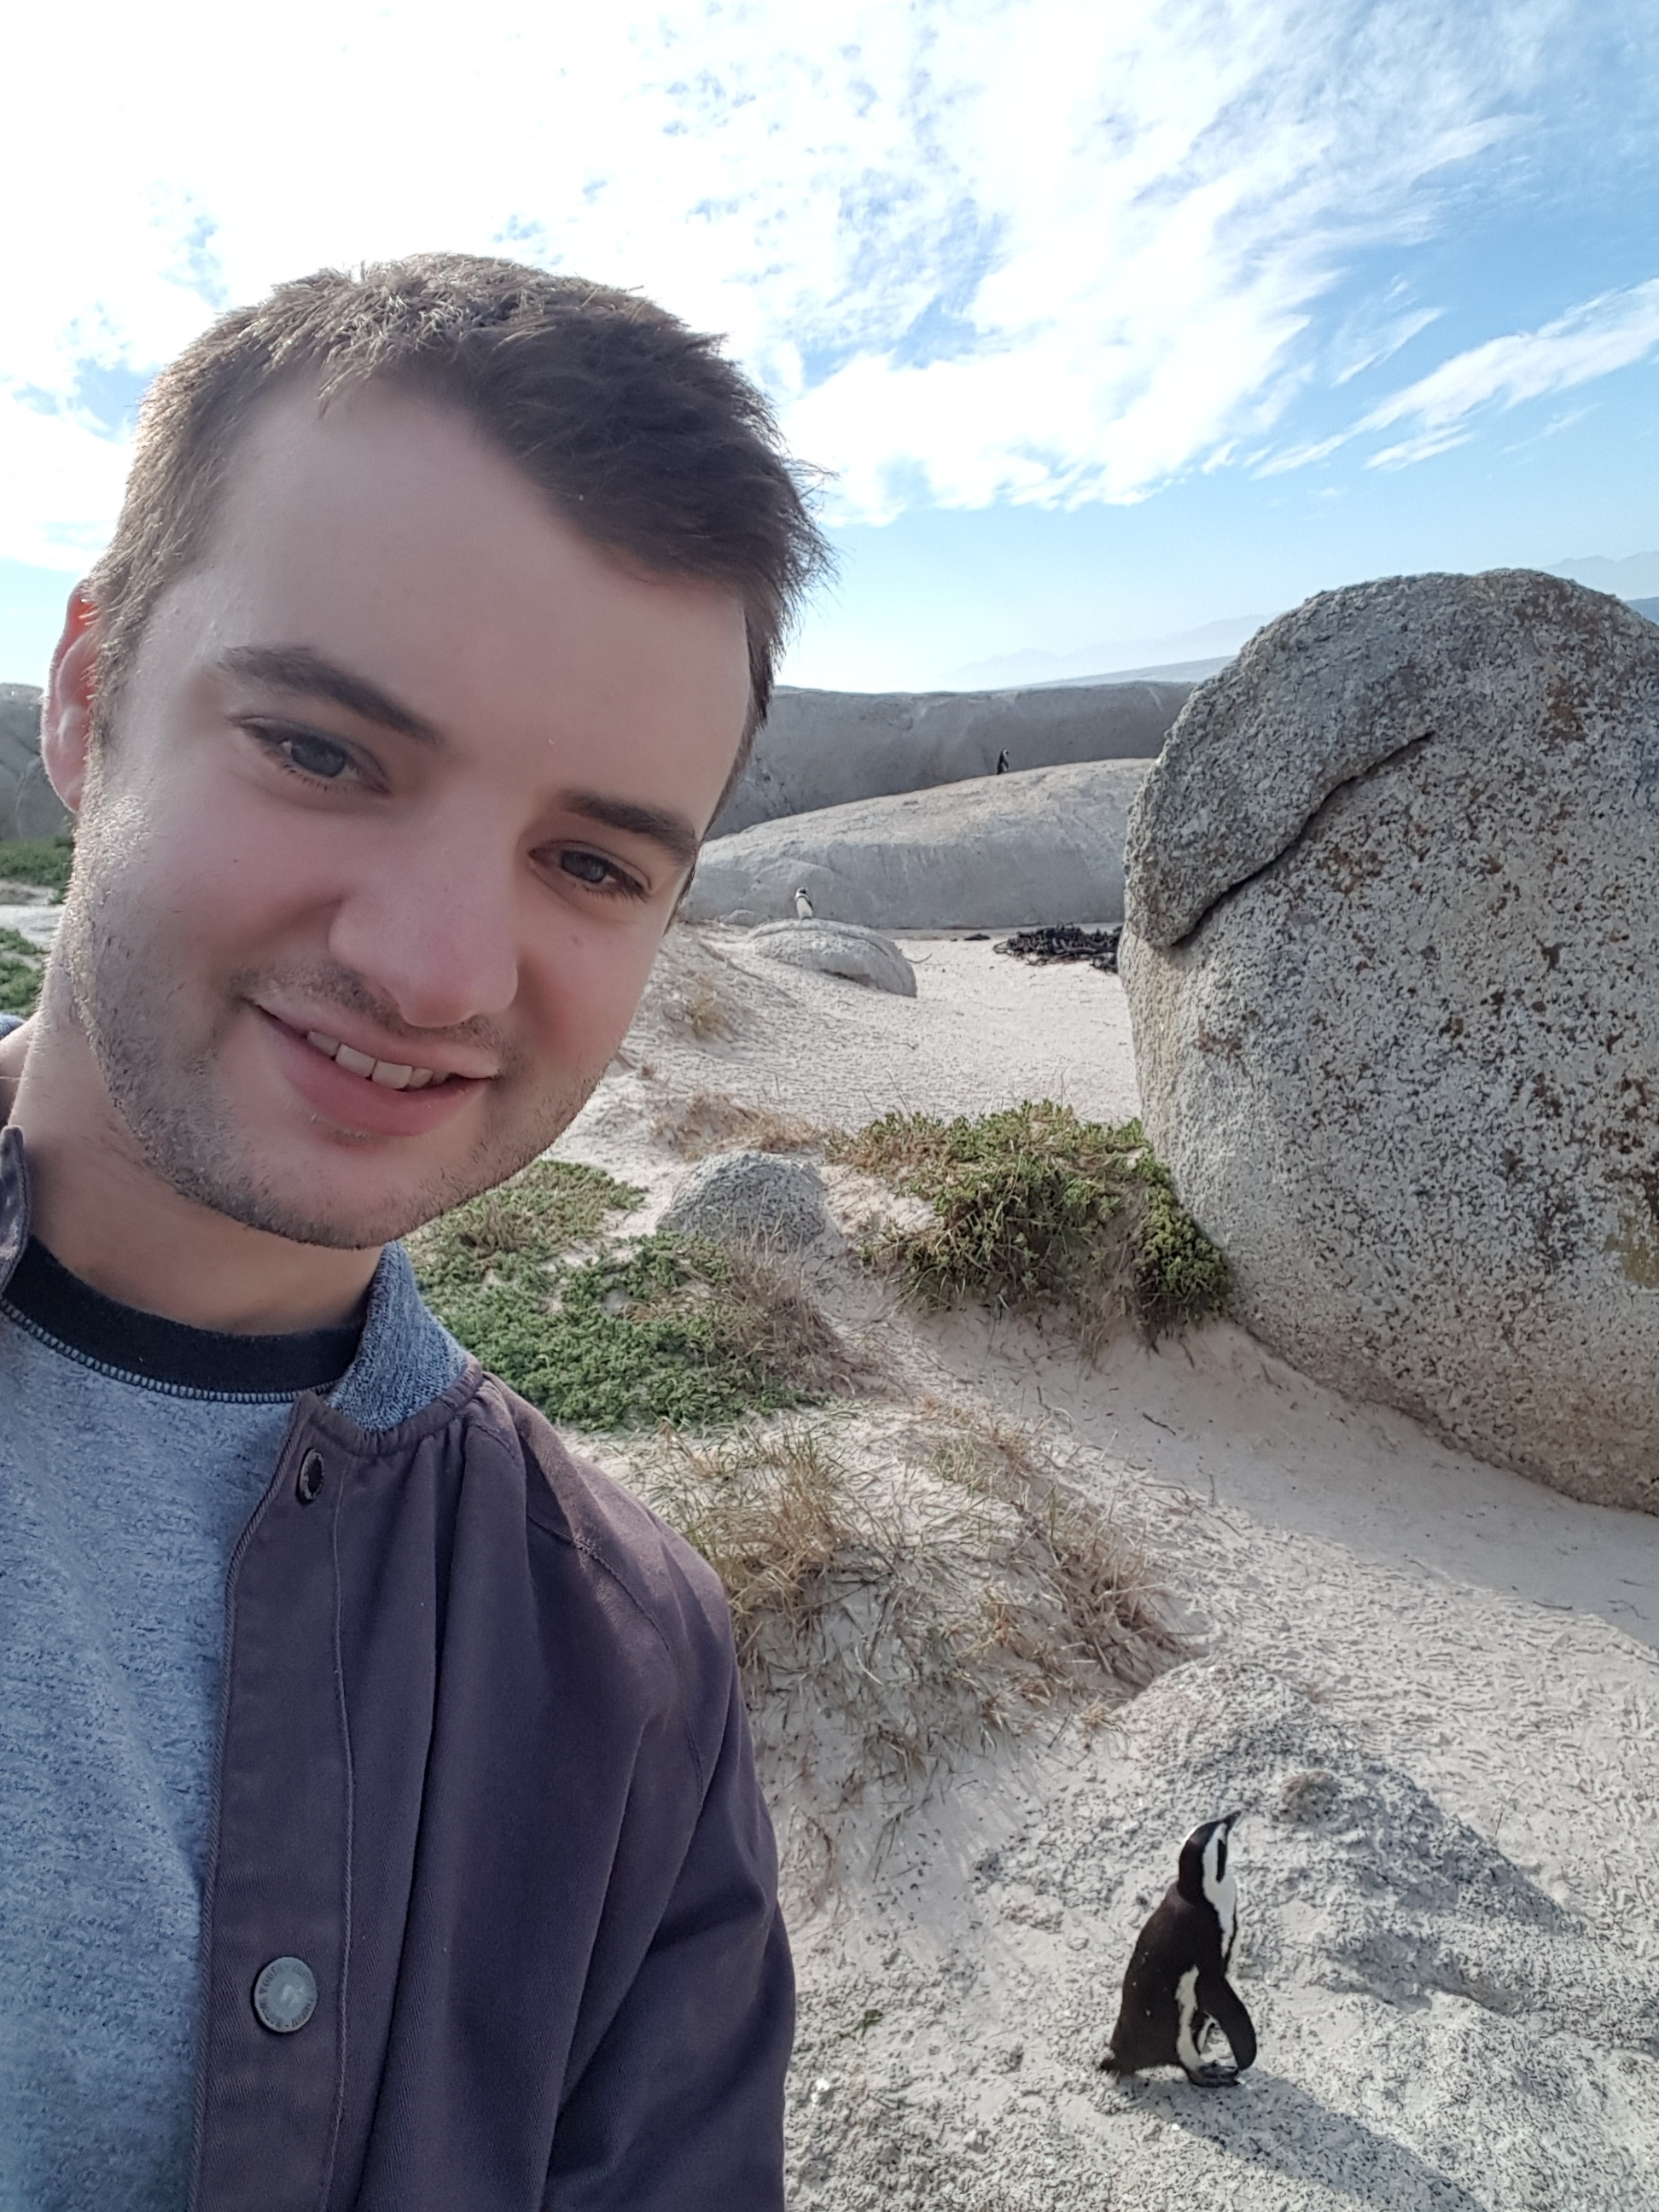
\includegraphics[width=0.35\textwidth]{IMAGES/MikePenguin}
%      };
%   \end{tikzpicture}
%      \titlepage
%\end{frame}
%%%%%%%%%%%%%%%%%%%%%%%%%%%%%%%%%%%%%%%%%%%%%%%%%

%%%%%%%%%%%%%%%%%%%%%%%%%%%%%%%%%%%%%%%%%%%%%%%%%
\begin{frame}
%\frametitle{Thank-you}
   \begin{tikzpicture}[overlay, remember picture]
%         \node[anchor = north, text width = 1.1\linewidth] at (current page.north) {
%	   Gametic selection, meiotic drive, sex ratio bias, and transitions b/w sex determination systems
%	 };     
         \node[anchor = south west, text width = 0.4\linewidth] at (current page.south west) {
   	    \centering
	    Michael Scott$^1$\\
	    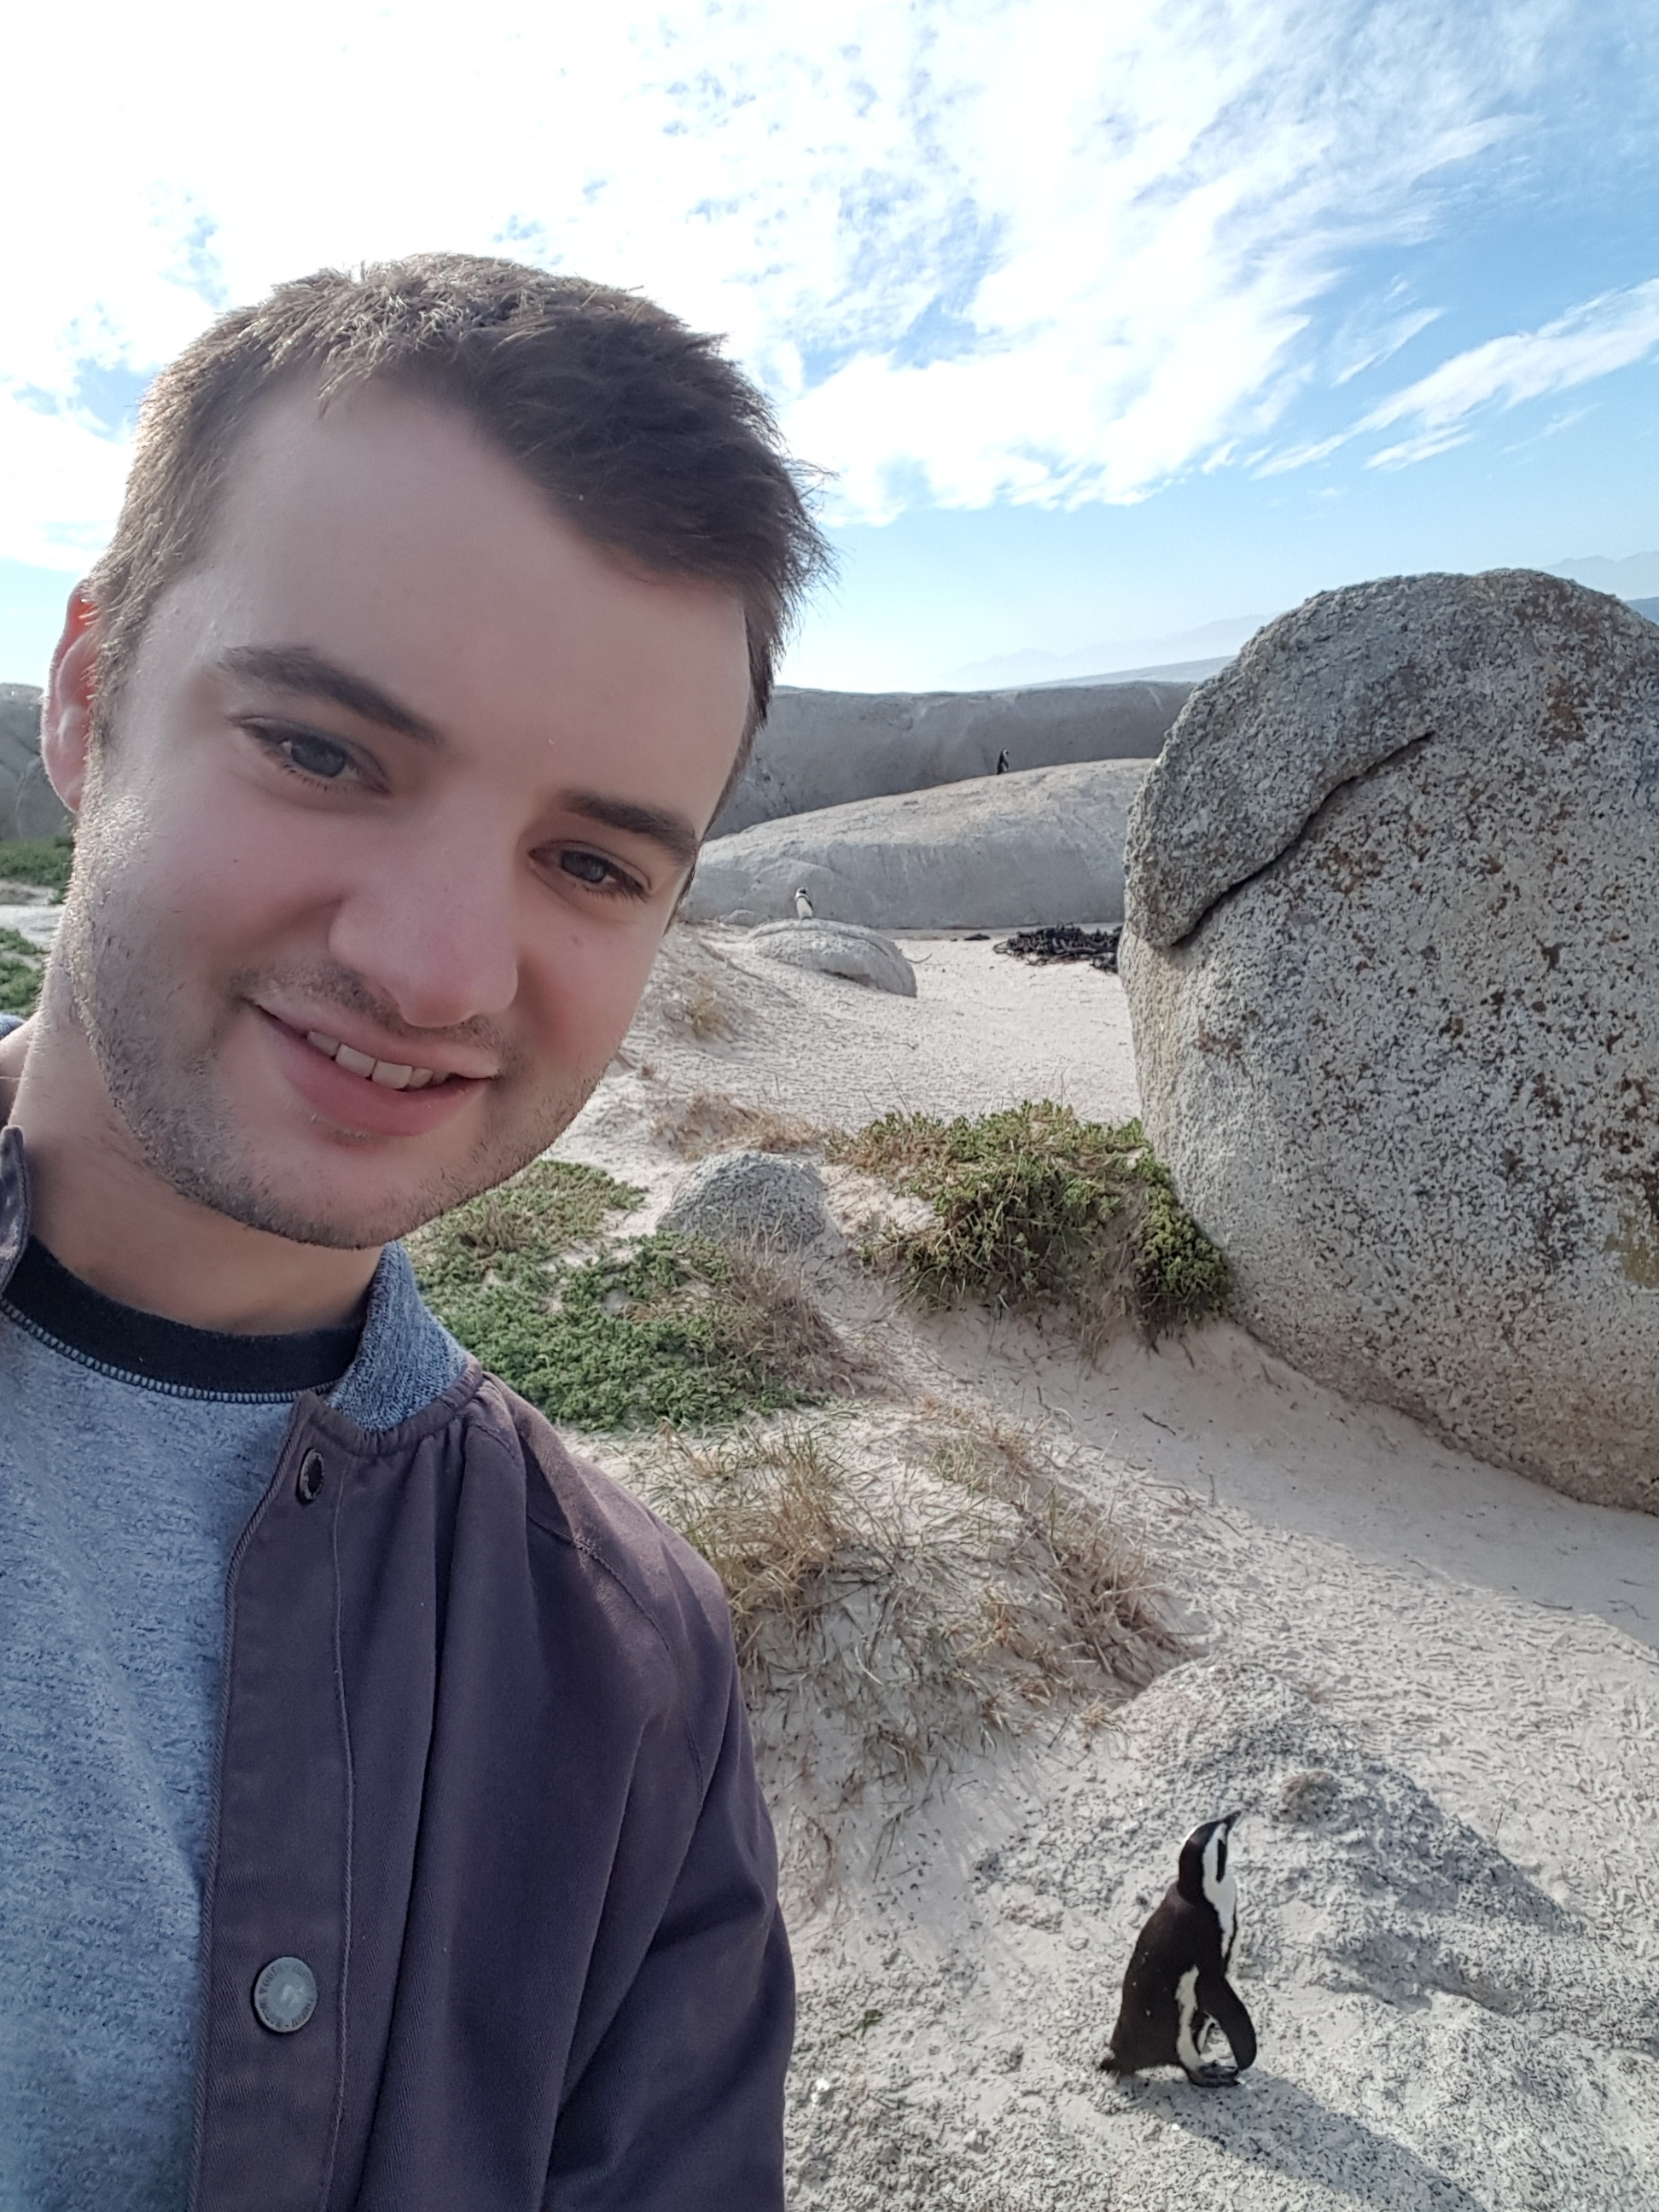
\includegraphics[trim = {0 35cm 0 0}, clip, width=\textwidth]{IMAGES/MikePenguin}
	 };            
         \node[anchor = south east, text width = 0.45\linewidth] at (current page.south east) {
   	    \centering
            Sally Otto$^2$\\
   	    \scalebox{-1}[1]{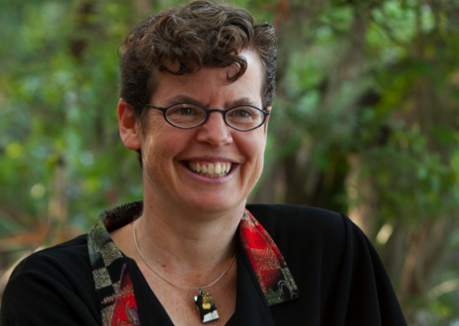
\includegraphics[width=\textwidth]{IMAGES/Sally}}
	 };     
%         \node[anchor = south west, yshift=0.7cm] at (current page.south west) {
%   	    
\includegraphics[width=0.5\textwidth]{IMAGES/BRC}
%	 };     
%         \node[anchor = south, xshift=1cm] at (current page.south) {
%	    
\includegraphics[width=0.15\textwidth]{IMAGES/UBC}
%	 };     
%         \node[anchor = south east, yshift=0.5cm] at (current page.south east) {	    			   
\includegraphics[width=0.3\textwidth]{IMAGES/NSERC}
%	 };   	   
   \end{tikzpicture}
   \titlepage
\end{frame}
%%%%%%%%%%%%%%%%%%%%%%%%%%%%%%%%%%%%%%%%%%%%%%%%%

%%%%%%%%%%%%%%%%%%%%%%%%%%%%%%%%%%%%%%%%%%%%%%%%%
\begin{frame}
\frametitle{Sex determination systems are remarkably dynamic}
   \begin{tikzpicture}[overlay, remember picture]
\visible<1>{
      \node[anchor = center] at (current page.center) {
         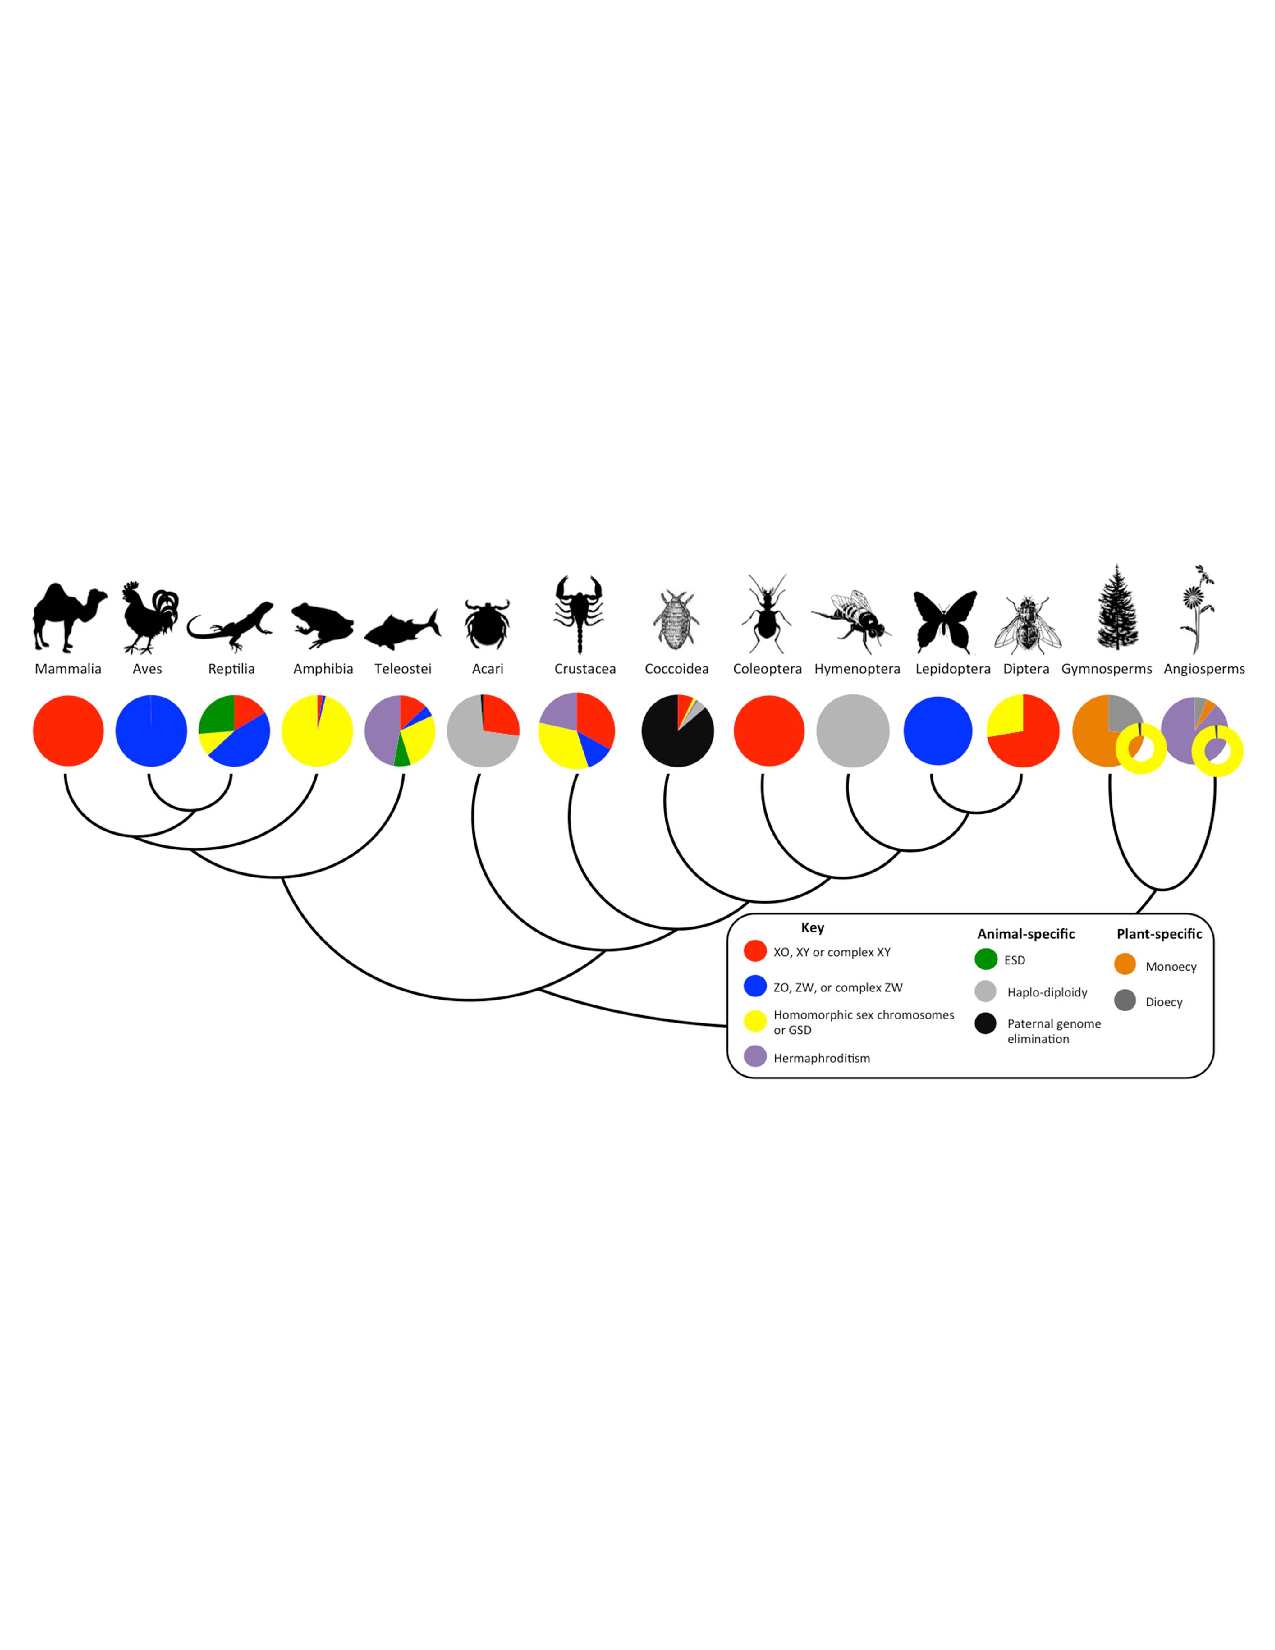
\includegraphics[width=\linewidth, angle=0]{IMAGES/BachtrogEtAl2014Fig3}
      };
      \node[anchor = south east] at (current page.south east) {
         Bachtrog \textit{et al.} 2014
      };
      \node[anchor = center, yshift=-4cm] at (current page.center) {
         
\includegraphics[width=\linewidth, angle=0]{IMAGES/BachtrogEtAl2014Title}
      };
}
\visible<2->{
         \node[anchor = center] at (current page.center) {
           \huge 2 theories
	};
}
   \end{tikzpicture}
\end{frame}
%%%%%%%%%%%%%%%%%%%%%%%%%%%%%%%%%%%%%%%%%%%%%%%%%

%%%%%%%%%%%%%%%%%%%%%%%%%%%%%%%%%%%%%%%%%%%%%%%%%
\begin{frame}
\frametitle{\underline{Theory 1}: Turnover caused by \textcolor{red}{sex-ratio selection}}
   \begin{tikzpicture}[overlay, remember picture]
\visible<2>{
      \node[anchor = east, text width = 0.5\linewidth, xshift=-0.5cm] at (current page.east) {
         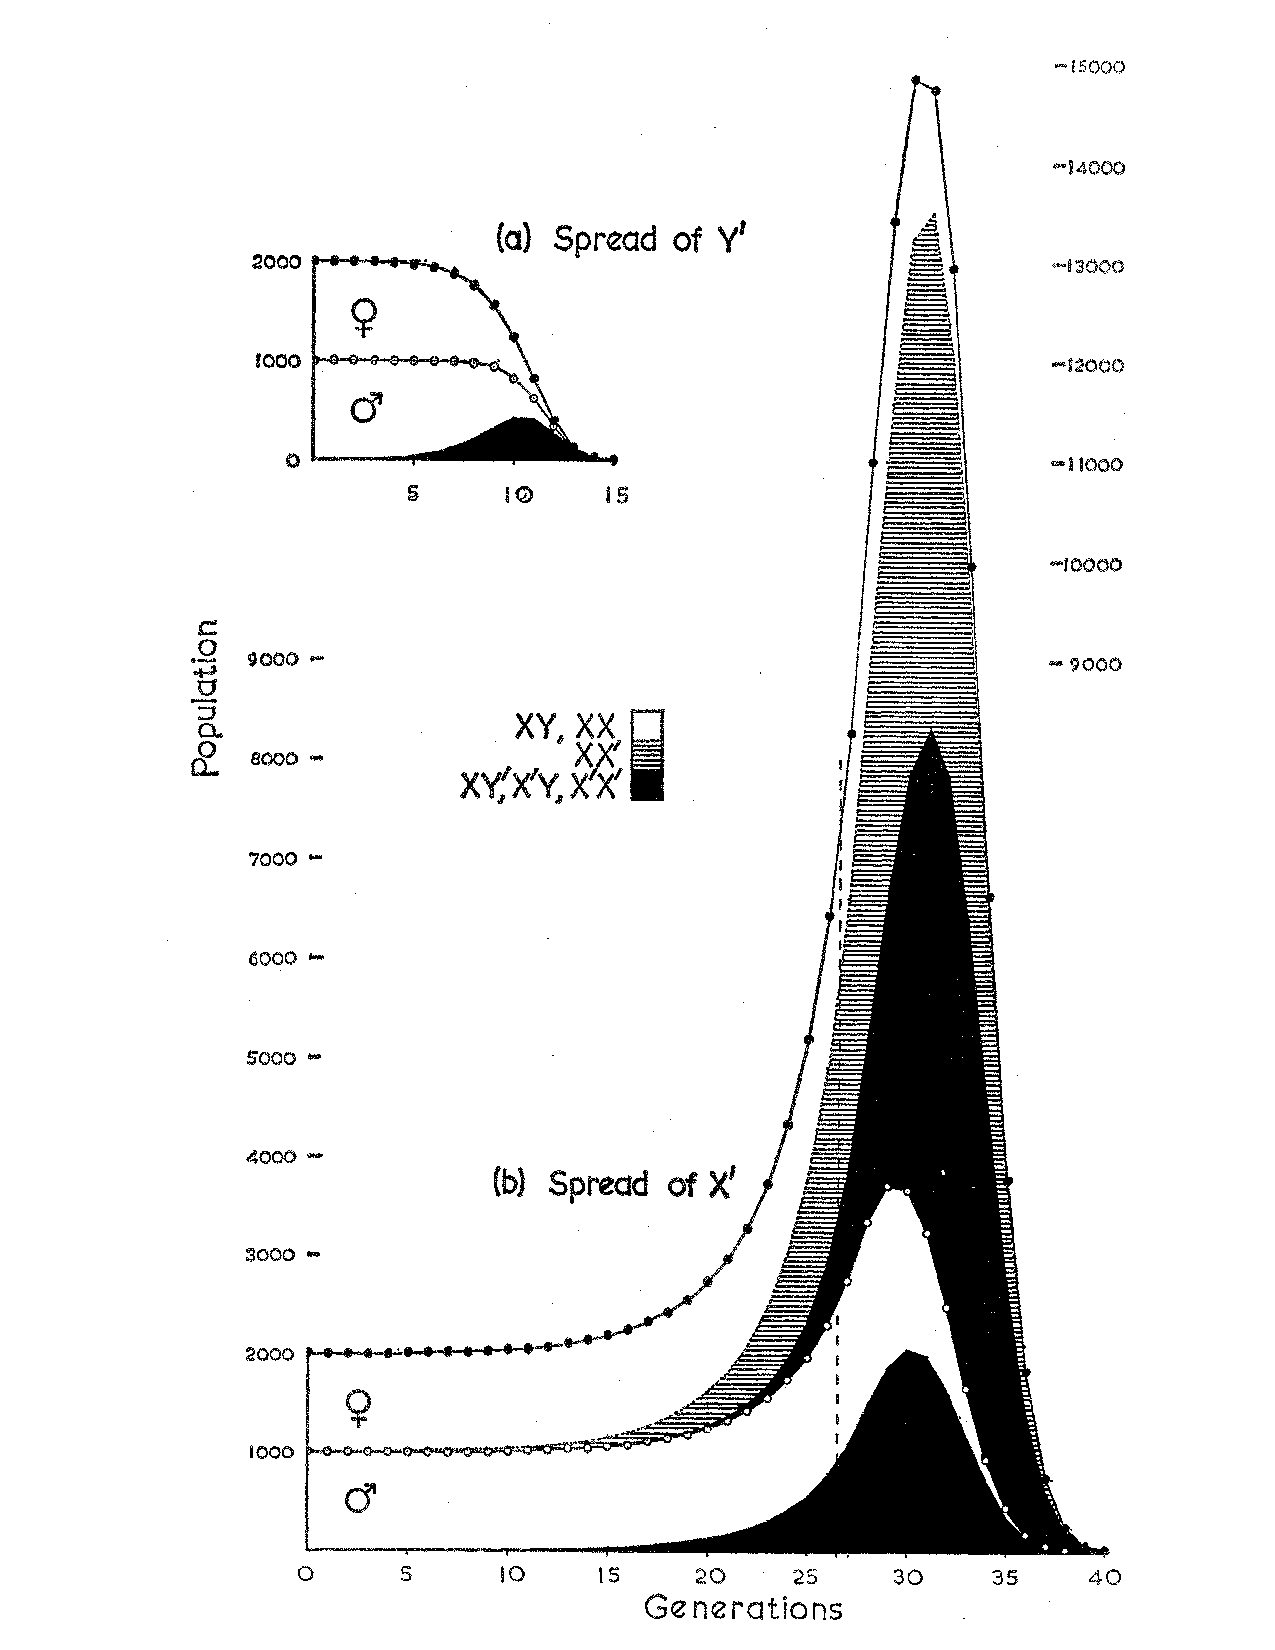
\includegraphics[width=\linewidth, angle=0]{IMAGES/Hamilton1967Fig1}
      };
      \node[anchor = east, text width = 0.5\linewidth, yshift = -4cm, xshift=0cm] at (current page.east) {
         
\includegraphics[width=\linewidth, angle=0]{IMAGES/Hamilton1967Title}
      };
}
\visible<2->{
      \node[anchor = south west] at (current page.south west) {
         Hamilton 1967
      };
      \node[anchor = west, text width = 0.5\linewidth, xshift = 20, yshift = 0] at (current page.west) {
         \huge Meiotic-drive for $Y$\\\vspace{0.1cm} increases $\male:\female$
      };
}
\visible<3->{
%      \node[anchor = east, text width = 0.75\linewidth, yshift=-1.5cm] at (current page.east) {
%         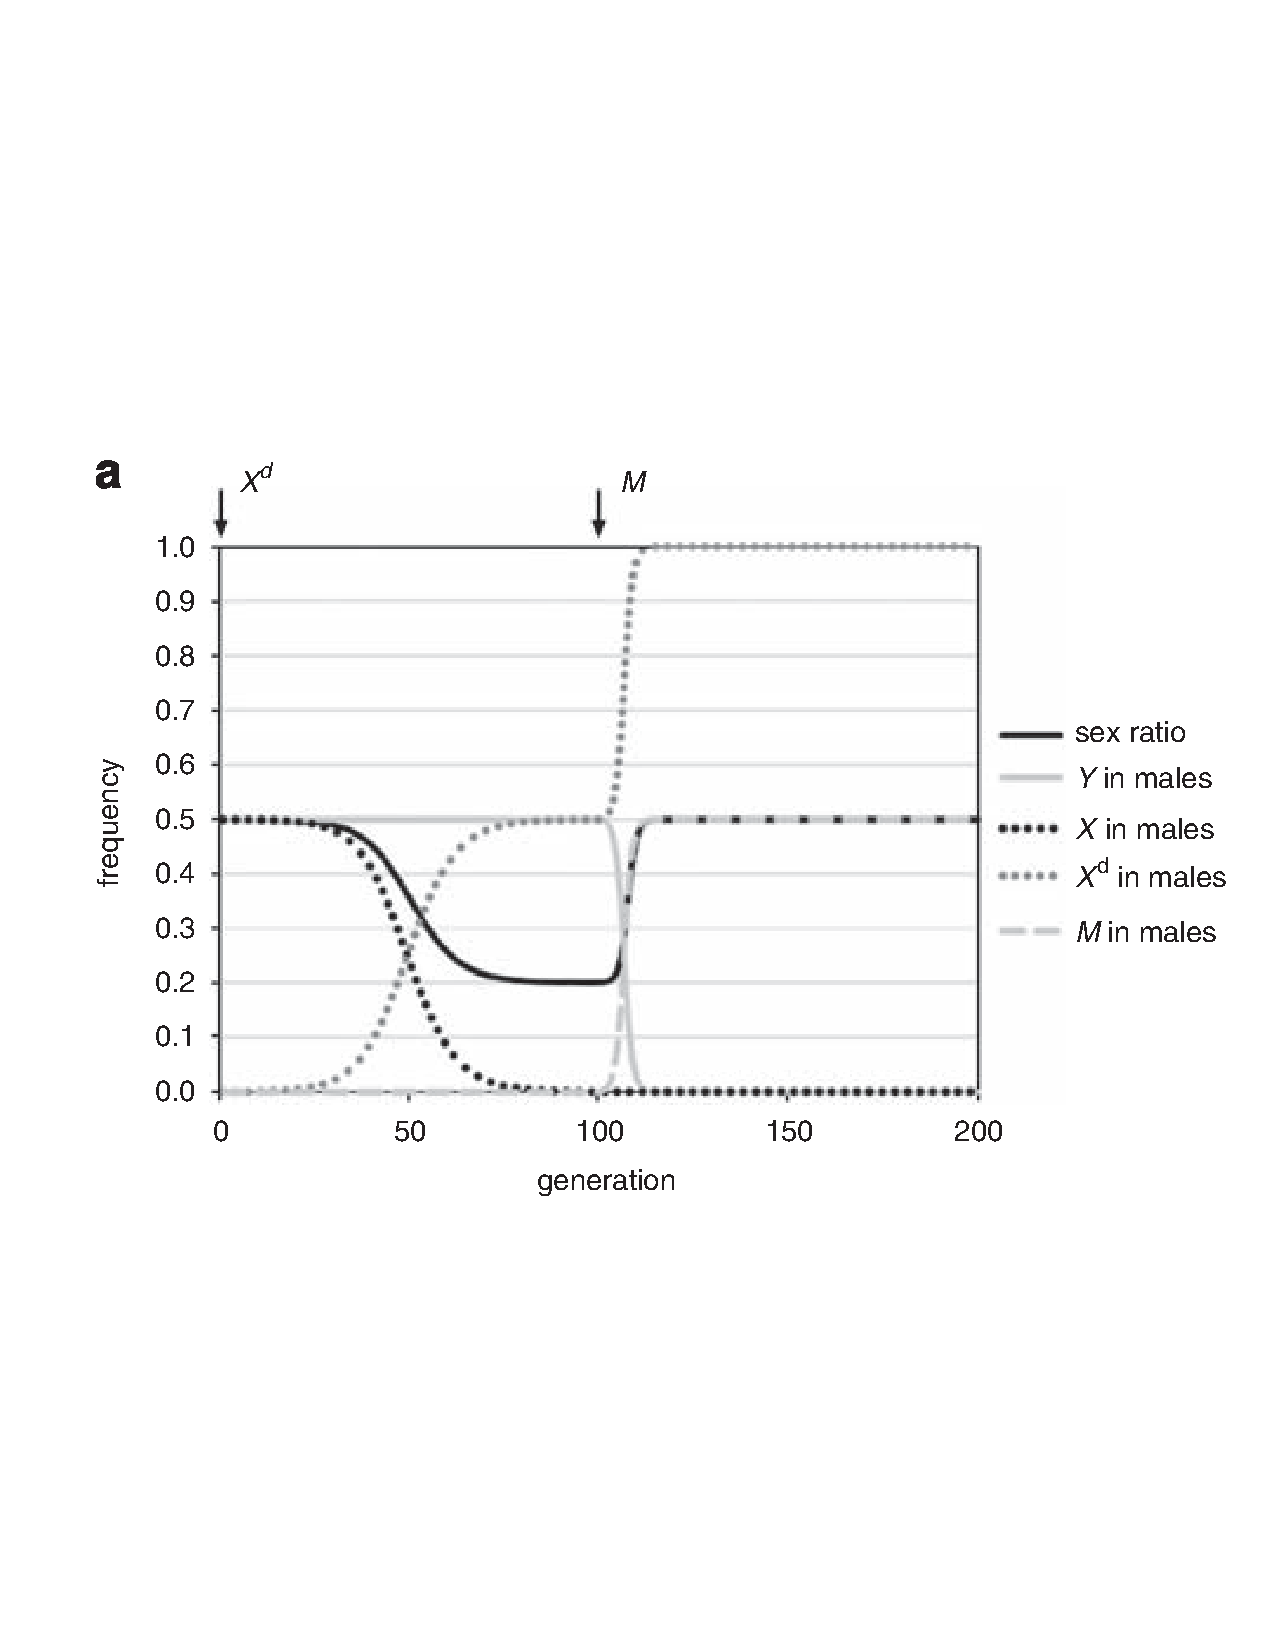
\includegraphics[width=\linewidth, angle=0]{IMAGES/KozielskaEtAl2010Fig1a}
%      };
%      \node[anchor = east, text width = 0.7\linewidth, yshift = 2cm] at (current page.east) {
%         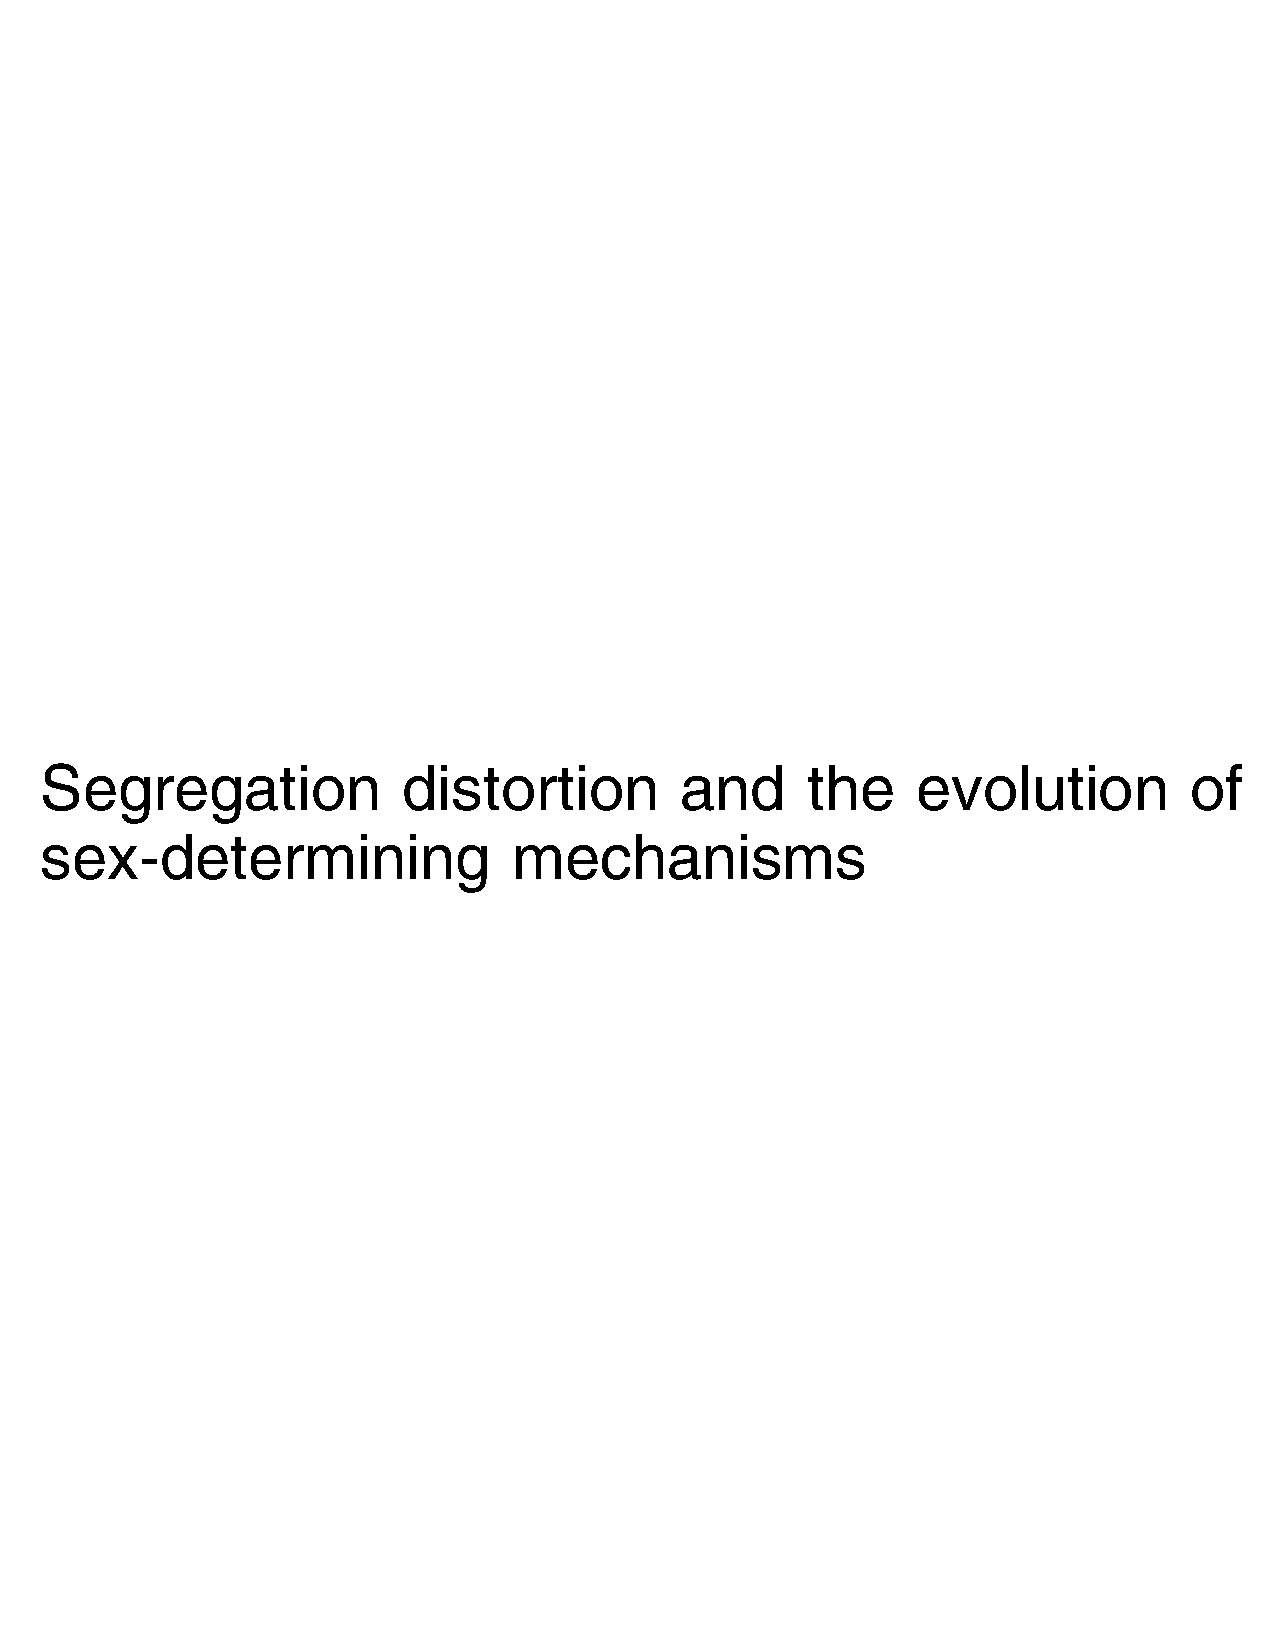
\includegraphics[width=\linewidth, angle=0]{IMAGES/KozielskaEtAl2010Title}
%      };
      \node[anchor = south east, yshift=0cm] at (current page.south east) {
         Kozielska \textit{et al.} 2010
      };
      \node[anchor = east, text width = 0.4\linewidth, xshift = -20, yshift = 0] at (current page.east) {
         \textcolor{blue}{\huge neo-$W$ restores\\\vspace{0.1cm} $1:1$ sex ratio}
      };
      \node[anchor = center, text width = 0.4\linewidth, xshift = 0, yshift = -60] at (current page.center) {
         \huge $X Y \rightarrow \textcolor{blue}{Z W}$
      };
 }
%\visible<4->{
%      \node[anchor = west, text width = 0.4\linewidth, xshift = 20, yshift = -90] at (current page.west) {
%         \textcolor{gray}{\huge $X Y^d \rightarrow ZW$}
%      };
%}
   \end{tikzpicture}
\end{frame}
%%%%%%%%%%%%%%%%%%%%%%%%%%%%%%%%%%%%%%%%%%%%%%%%%

%%%%%%%%%%%%%%%%%%%%%%%%%%%%%%%%%%%%%%%%%%%%%%%%%
\begin{frame}
\frametitle{\underline{Theory 2}: Turnover caused by \textcolor{red}{sex-antagonistic selection}}
   \begin{tikzpicture}[overlay, remember picture]
\visible<1->{
      \node[anchor = south east] at (current page.south east) {
         van Doorn \& Kirkpatrick 2010
      };
      \node[anchor = center, xshift= -30, yshift = 70] at (current page.center) {
         \huge $XY \rightarrow \textcolor{blue}{ZW}$
      };   
}
   %chromosomal order (move coordinate C and position of locus A only)  
%   \coordinate (C) at (5.5,-2); 
%   \coordinate (A) at ($(C)+(1.5,0)$); 
%   \draw[thick] (C) -- ($(C)+(2.5,0)$);
%   \draw[thick] ($(A)+(0,-0.1)$) -- ($(A)+(0,0.1)$) node[above] {$\textcolor{red}{A}$};
%   \draw[thick] ($(C)+(1,-0.1)$) -- ($(C)+(1,0.1)$) node[above] {$Y$};
%   \draw[thick] ($(C)+(2,-0.1)$) -- ($(C)+(2,0.1)$) node[above] {$\textcolor{blue}{W}$};
\visible<2-4>{
   %chromosomal order (move coordinate C and position of locus A only)  
   \coordinate (C) at (7.5,2);
   \coordinate (A) at ($(C)+(2.5,0)$); 
   \draw[thick] (C) -- ($(C)+(3,0)$);
   \draw[thick] ($(A)+(0,-0.1)$) -- ($(A)+(0,0.1)$) node[above] {$\textcolor{red}{A}$};
   \draw[thick] ($(C)+(1,-0.1)$) -- ($(C)+(1,0.1)$) node[above] {$Y$};
   \draw[thick] ($(C)+(2,-0.1)$) -- ($(C)+(2,0.1)$) node[above] {$\textcolor{blue}{W}$};   
}
\visible<2-3>{
   \node[anchor = center, xshift= 0, yshift = 0] at (current page.center) {
      \huge e.g., $\textcolor{red}{a}$ favoured in $\male$, $\textcolor{red}{A}$ favoured in $\female$
   };   
}
\visible<3-4>{
   %chromosomal order (move coordinate C and position of locus A only)  
   \coordinate (C) at (2.35,-2);
   \coordinate (A) at ($(C)+(0.5,0)$); 
   \draw[thick] (C) -- ($(C)+(2.5,0)$);
   \draw[thick] ($(A)+(0,-0.1)$) -- ($(A)+(0,0.1)$) node[above] {$\textcolor{red}{A}$};
   \draw[thick] ($(C)+(1,-0.1)$) -- ($(C)+(1,0.1)$) node[above] {$Y$};
   \draw[thick] ($(C)+(2,-0.1)$) -- ($(C)+(2,0.1)$) node[above] {$\textcolor{blue}{W}$};
}
\visible<4>{
      \node[anchor = center, yshift = -10] at (current page.center) {
         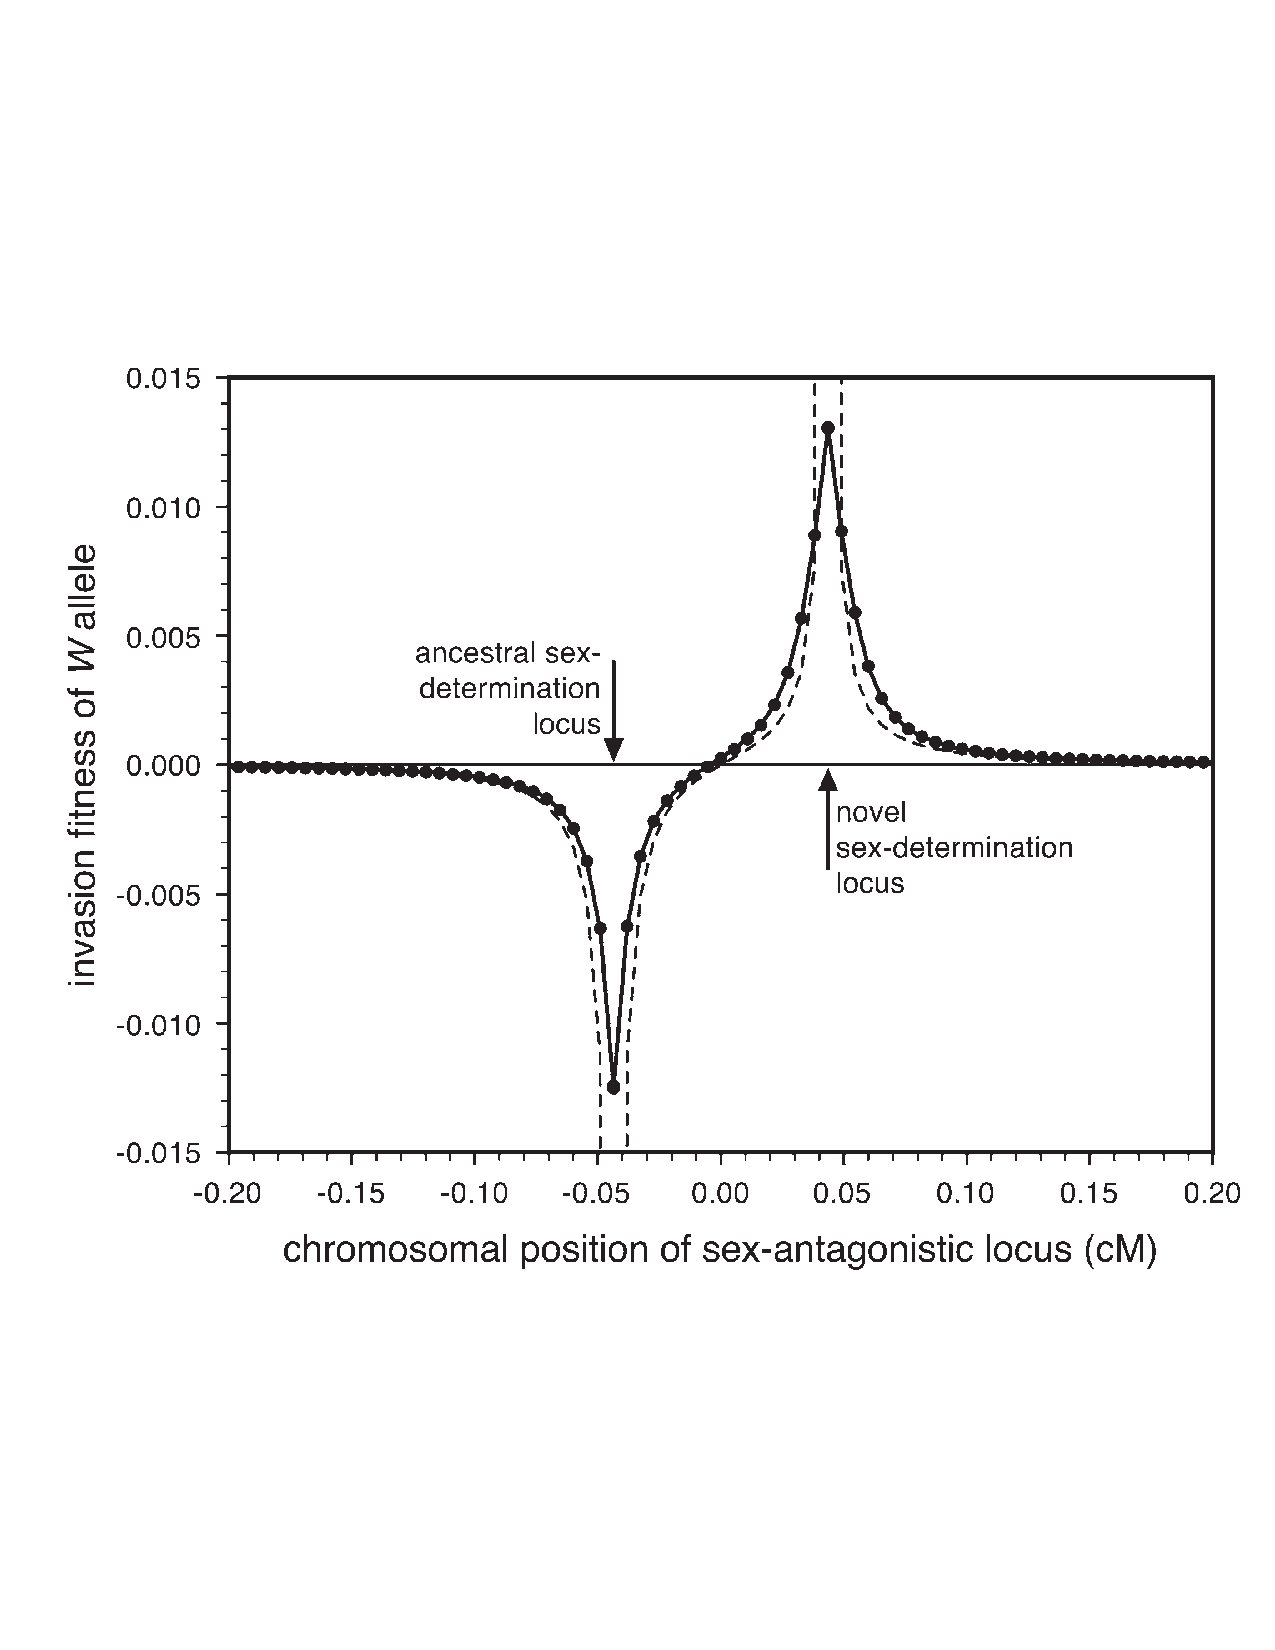
\includegraphics[width=0.9\linewidth, angle=0]{IMAGES/vanDoornKirkpatrick2010Fig2}
      };
      \node[anchor = center, xshift= 122, yshift = -102] at (current page.center) {
         ($\textcolor{red}{A}$)
      };         
      \node[anchor = center, xshift= -60, yshift = 20] at (current page.center) {
         ($\textcolor{black}{Y}$)
      };    
      \node[anchor = center, xshift= 110, yshift = -15] at (current page.center) {
         ($\textcolor{blue}{W}$)
      };
     \draw [decorate,decoration={brace,amplitude=10pt,raise=4pt},yshift=0pt,thick]
(1,0) -- (1,3) node [black,midway,xshift=-20,rotate=90] {\footnotesize
neo-$\textcolor{blue}{W}$ invades};     
}
%      \node[anchor = center, yshift=-3.9cm, xshift=0cm] at (current page.center) {
%         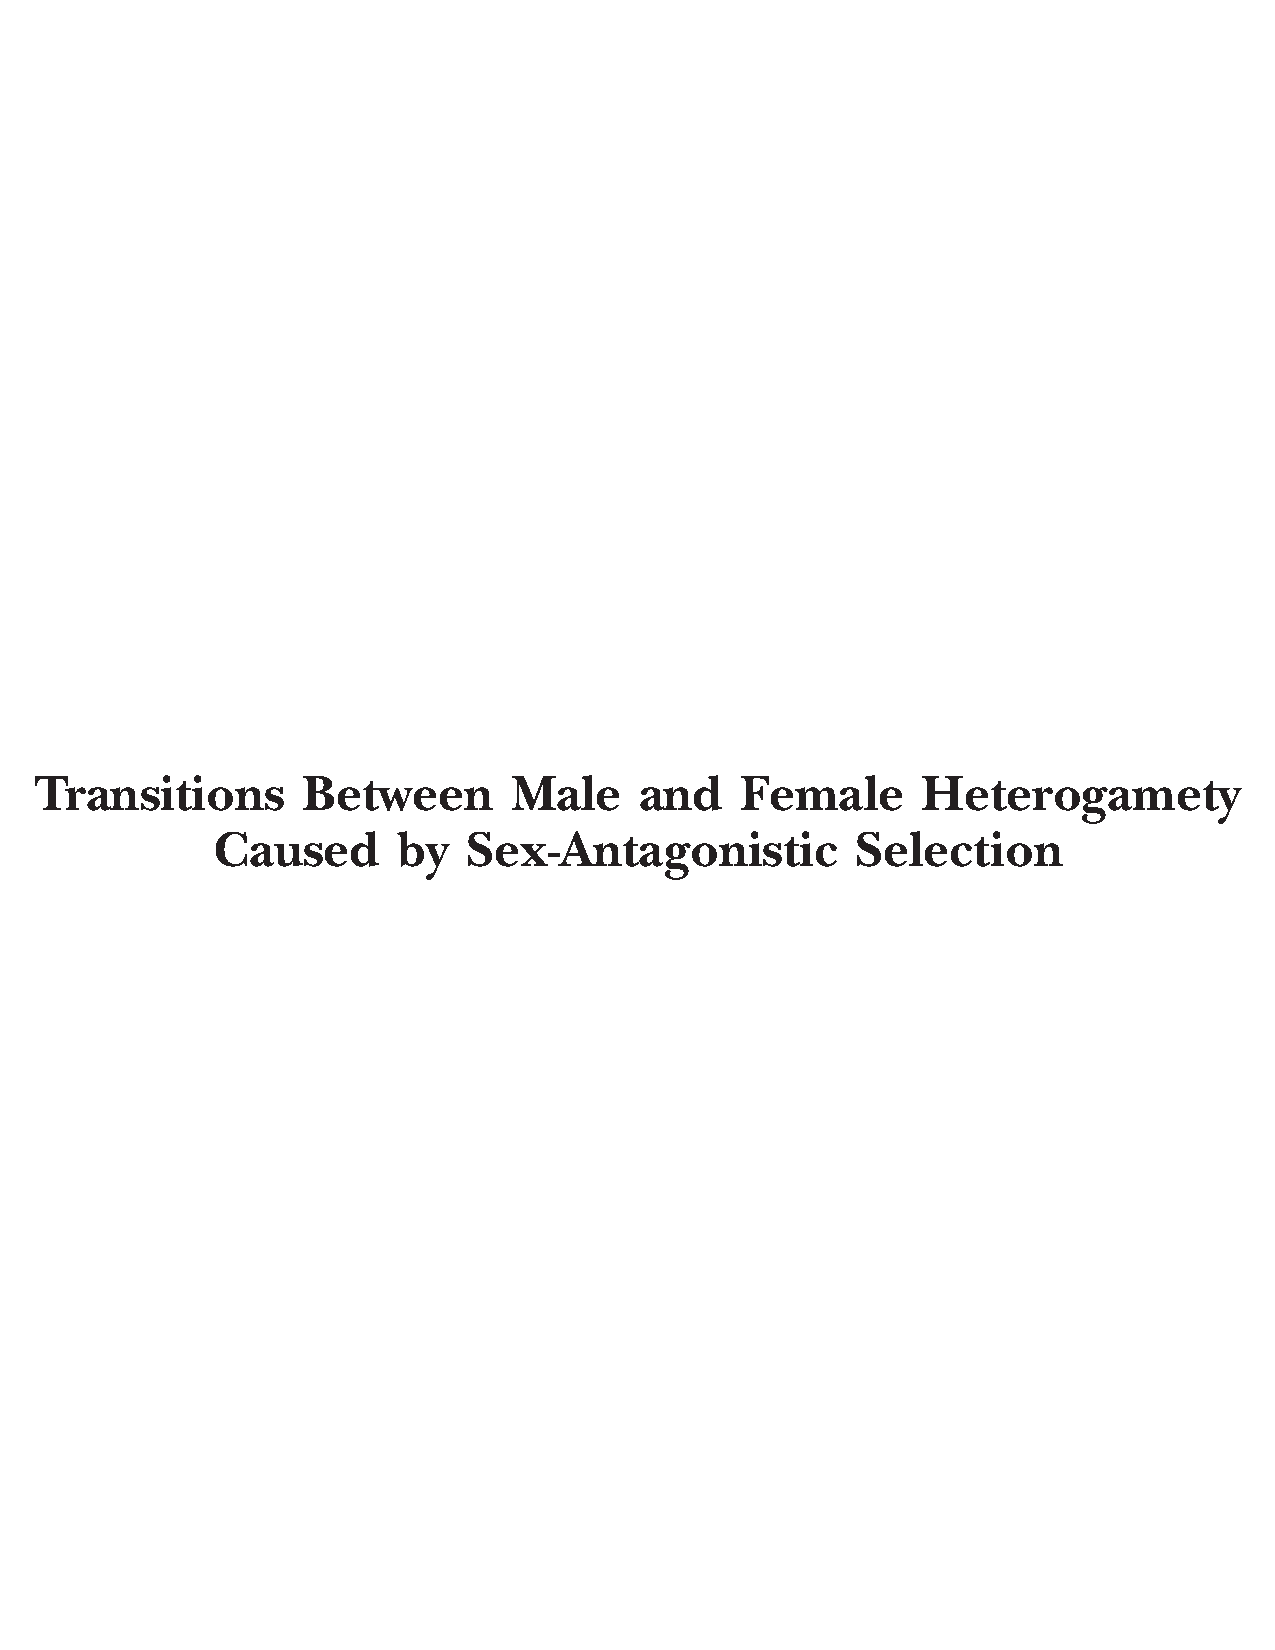
\includegraphics[width=0.9\linewidth, angle=0]{IMAGES/vanDoornKirkpatrick2010Title}
%      };
\visible<5->{
      \node[anchor = center, xshift= 0, yshift = 0] at (current page.center) {
         \huge turnover increases sex-linkage
      };
   %chromosomal order (move coordinate C and position of locus A only)  
   \coordinate (C) at (0,-2);
   \coordinate (A) at ($(C)+(2.5,0)$); 
   \draw[thick] (C) -- ($(C)+(3,0)$);
   \draw[thick] ($(A)+(0,-0.1)$) -- ($(A)+(0,0.1)$) node[above] {$\textcolor{red}{A}$};
   \draw[thick] ($(C)+(1,-0.1)$) -- ($(C)+(1,0.1)$) node[above] {$Y$};
%   \draw[thick] ($(C)+(2,-0.1)$) -- ($(C)+(2,0.1)$) node[above] {$\textcolor{blue}{W}$};  
      \node[anchor = center, xshift= 0, yshift = -50] at (current page.center) {
         \huge $\rightarrow$
      };   
   %chromosomal order (move coordinate C and position of locus A only)  
   \coordinate (C) at (7.5,-2);
   \coordinate (A) at ($(C)+(2.5,0)$); 
   \draw[thick] (C) -- ($(C)+(3,0)$);
   \draw[thick] ($(A)+(0,-0.1)$) -- ($(A)+(0,0.1)$) node[above] {$\textcolor{red}{A}$};
%   \draw[thick] ($(C)+(1,-0.1)$) -- ($(C)+(1,0.1)$) node[above] {$Y$};
   \draw[thick] ($(C)+(2,-0.1)$) -- ($(C)+(2,0.1)$) node[above] {$\textcolor{blue}{W}$};  
}
\visible<6->{
      \node[anchor = center, xshift= 0, yshift = -90] at (current page.center) {
         \huge neo-$\textcolor{blue}{W}$ is a better sex-specialist
      };
}
   \end{tikzpicture}
\end{frame}
%%%%%%%%%%%%%%%%%%%%%%%%%%%%%%%%%%%%%%%%%%%%%%%%%

%%%%%%%%%%%%%%%%%%%%%%%%%%%%%%%%%%%%%%%%%%%%%%%%%
\begin{frame}
   \begin{tikzpicture}[overlay, remember picture]
         \node[anchor = center, text width = 1.1\linewidth] at (current page.center) {
           \begin{center}
              \huge Sex-ratio \textbf{vs.} sex-antagonistic selection
           \end{center}
	};
   \end{tikzpicture}
\end{frame}
%%%%%%%%%%%%%%%%%%%%%%%%%%%%%%%%%%%%%%%%%%%%%%%%%

%%%%%%%%%%%%%%%%%%%%%%%%%%%%%%%%%%%%%%%%%%%%%%%%%
\begin{frame}
\frametitle{Haploid-diploid life-cycles}
   \begin{tikzpicture}[overlay, remember picture]
\visible<1->{
      \node[anchor = center, xshift = -70, yshift=50] at (current page.center) {
	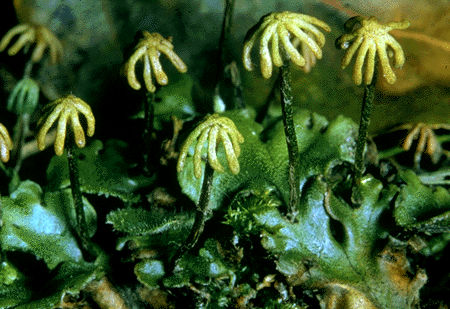
\includegraphics[width=0.4\linewidth]{IMAGES/Liverwort} %canadian encyclopedia, liverwort
      };
      \node[anchor = center, xshift = 60, yshift=65] at (current page.center) {
	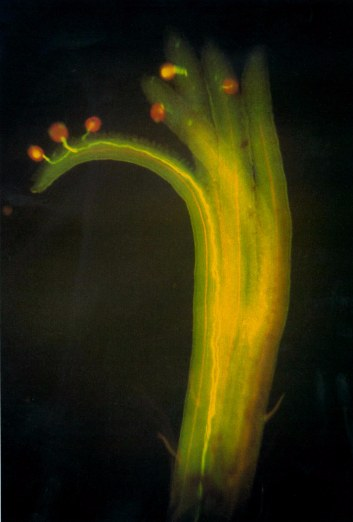
\includegraphics[width=0.25\linewidth]{IMAGES/Mulcahy01} %mulcahy & mulcahy 1987 Am Sci 75:44-50
      };
}
\visible<2->{
      \node[anchor = center, text width = 1.15\linewidth, yshift = -10] at (current page.center) {
	\textbf{Haploid selection (gametic competition \& meiotic drive)}
      };
}
\visible<3->{
      \node[anchor = center, text width = \linewidth, yshift=-40] at (current page.center) {
	Biased transmission of gametes, typically sex-specific\\
	$\implies$ can impart both \underline{sex-ratio \textbf{and} sex-antagonistic selection}
      };
}
\visible<4->{
      \node[anchor = center, text width = 1.15\linewidth, yshift=-70] at (current page.center) {
	Diploid selection too $\implies$ ploidally-antagonistic selection possible
      };
}
\visible<5->{
      \node[anchor = center, text width = 1.1\linewidth, yshift = -3.6cm] at (current page.center) {
         \begin{tcolorbox}[colback=blue!5!white,colframe=blue!75!black,title=Question]
	   How does haploid selection influence sex-determination turnover?
	\end{tcolorbox}	
      };
}
   \end{tikzpicture}
\end{frame}
%%%%%%%%%%%%%%%%%%%%%%%%%%%%%%%%%%%%%%%%%%%%%%%%%

%%%%%%%%%%%%%%%%%%%%%%%%%%%%%%%%%%%%%%%%%%%%%%%%%
\begin{frame}
\frametitle{Model}
   \begin{tikzpicture}[overlay, remember picture]
      \visible<1->{
         \node[anchor = east, text width = \linewidth, xshift=0.5cm] at (current page.east) {
	    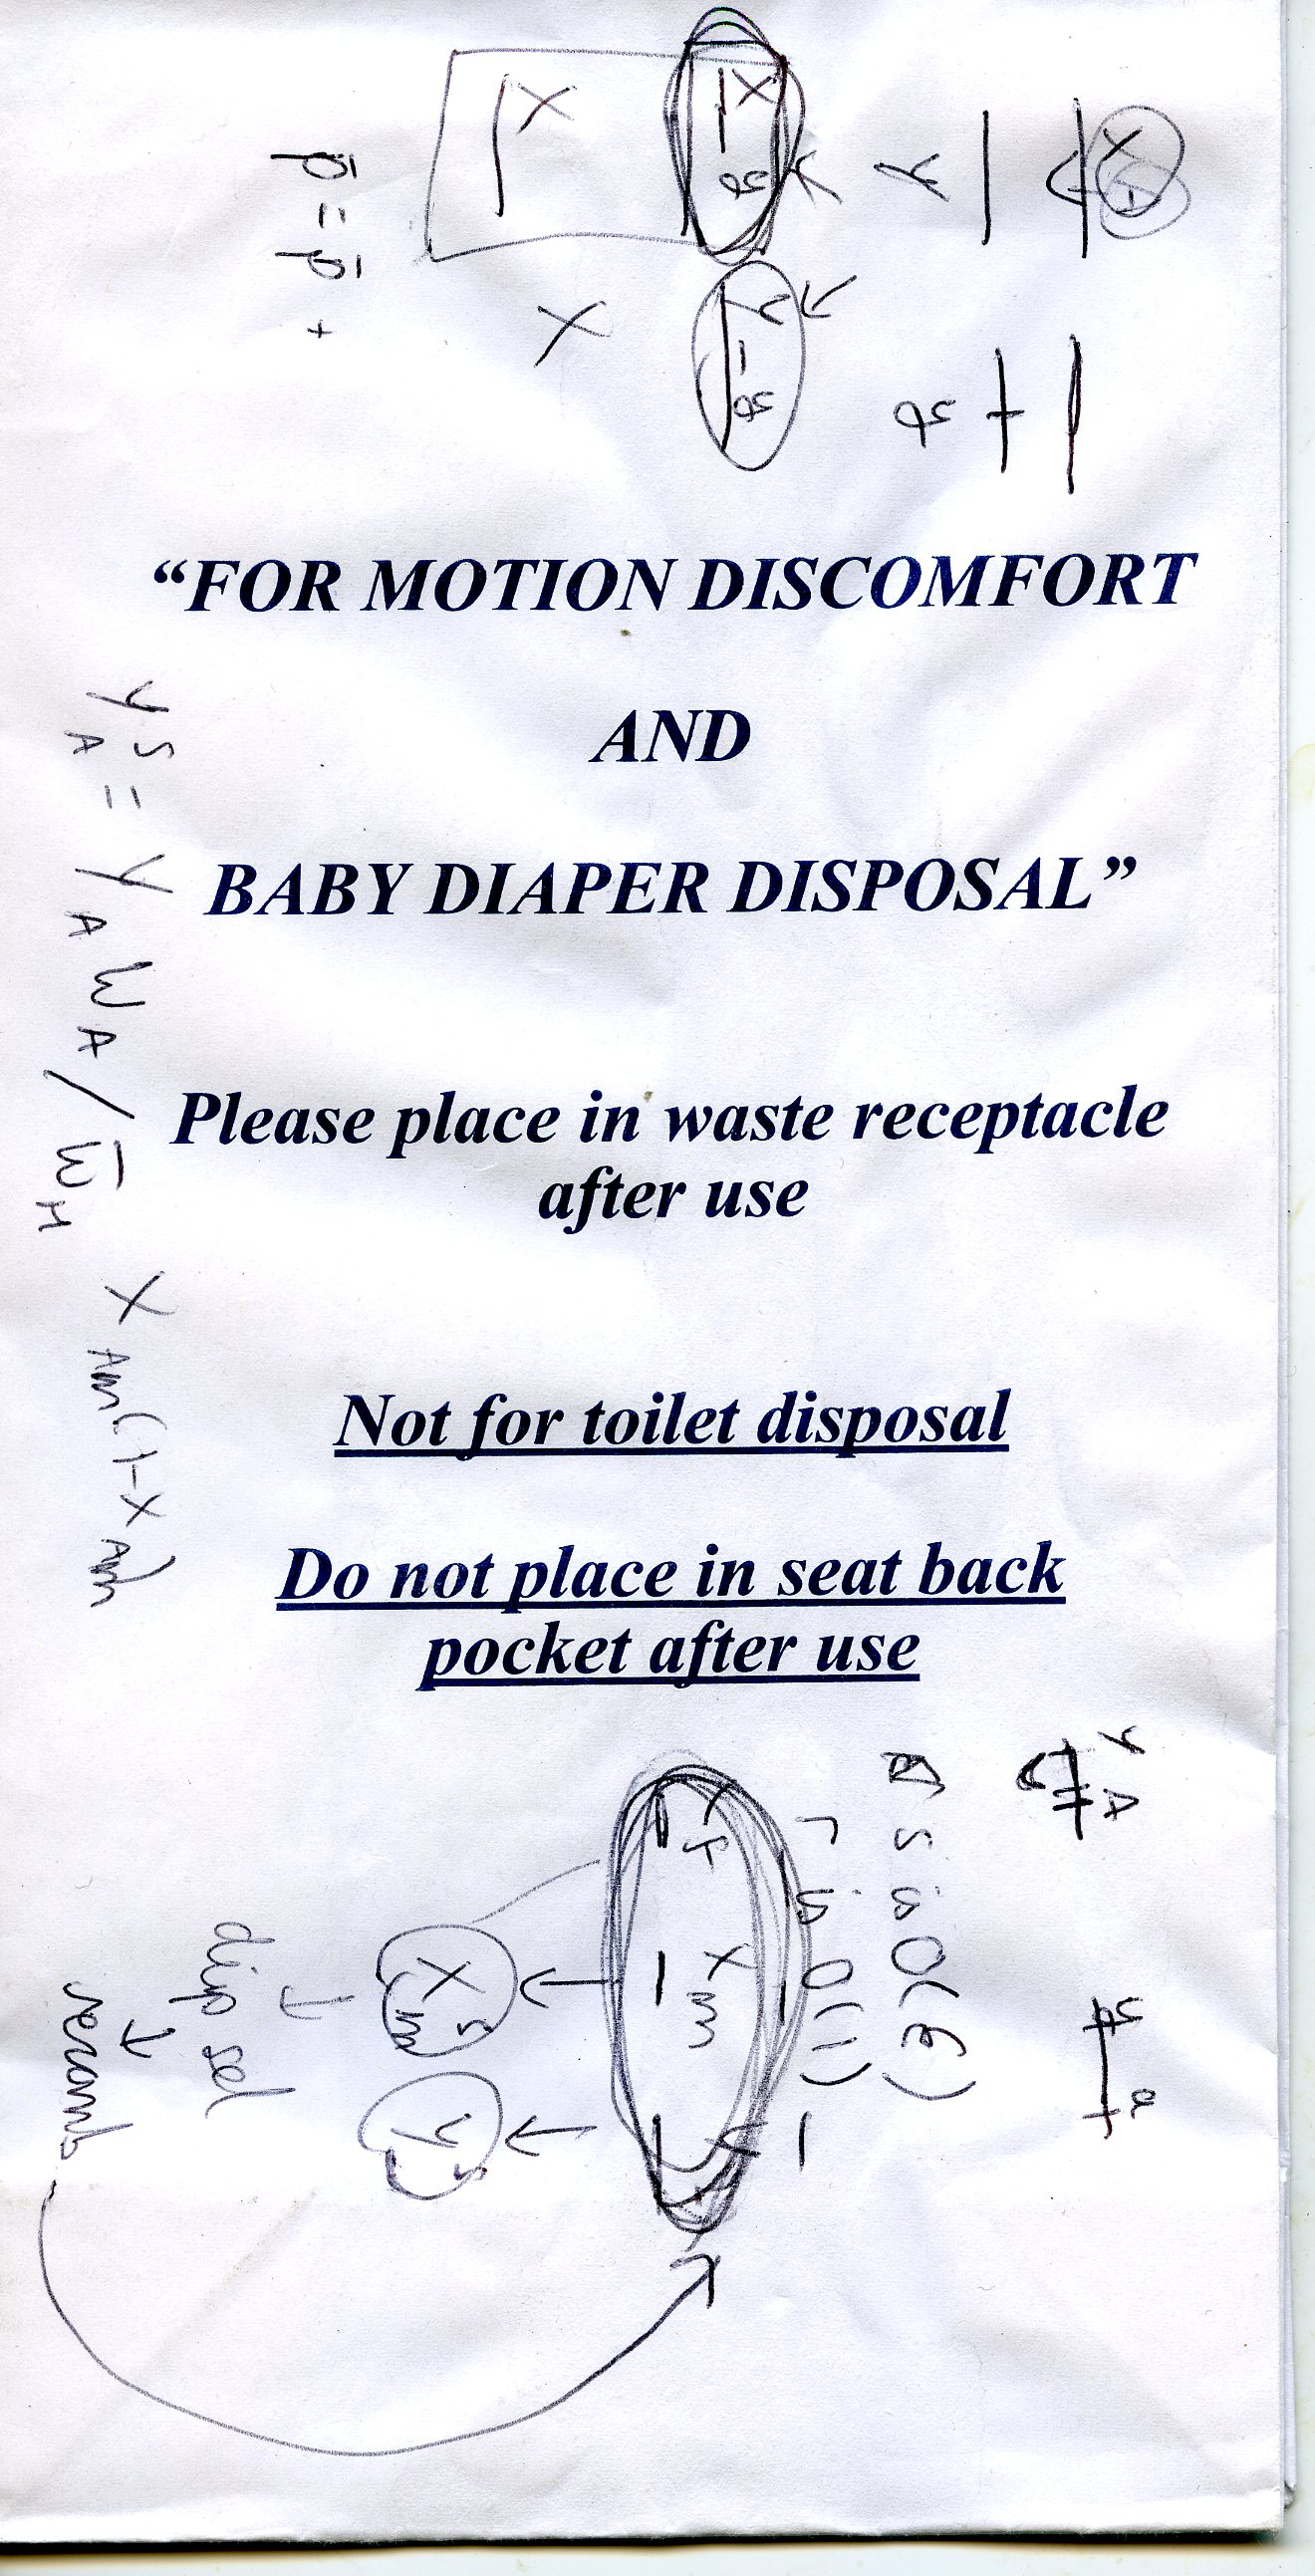
\includegraphics[width=0.4\linewidth, angle=90]{IMAGES/BarfBag1}\\
	    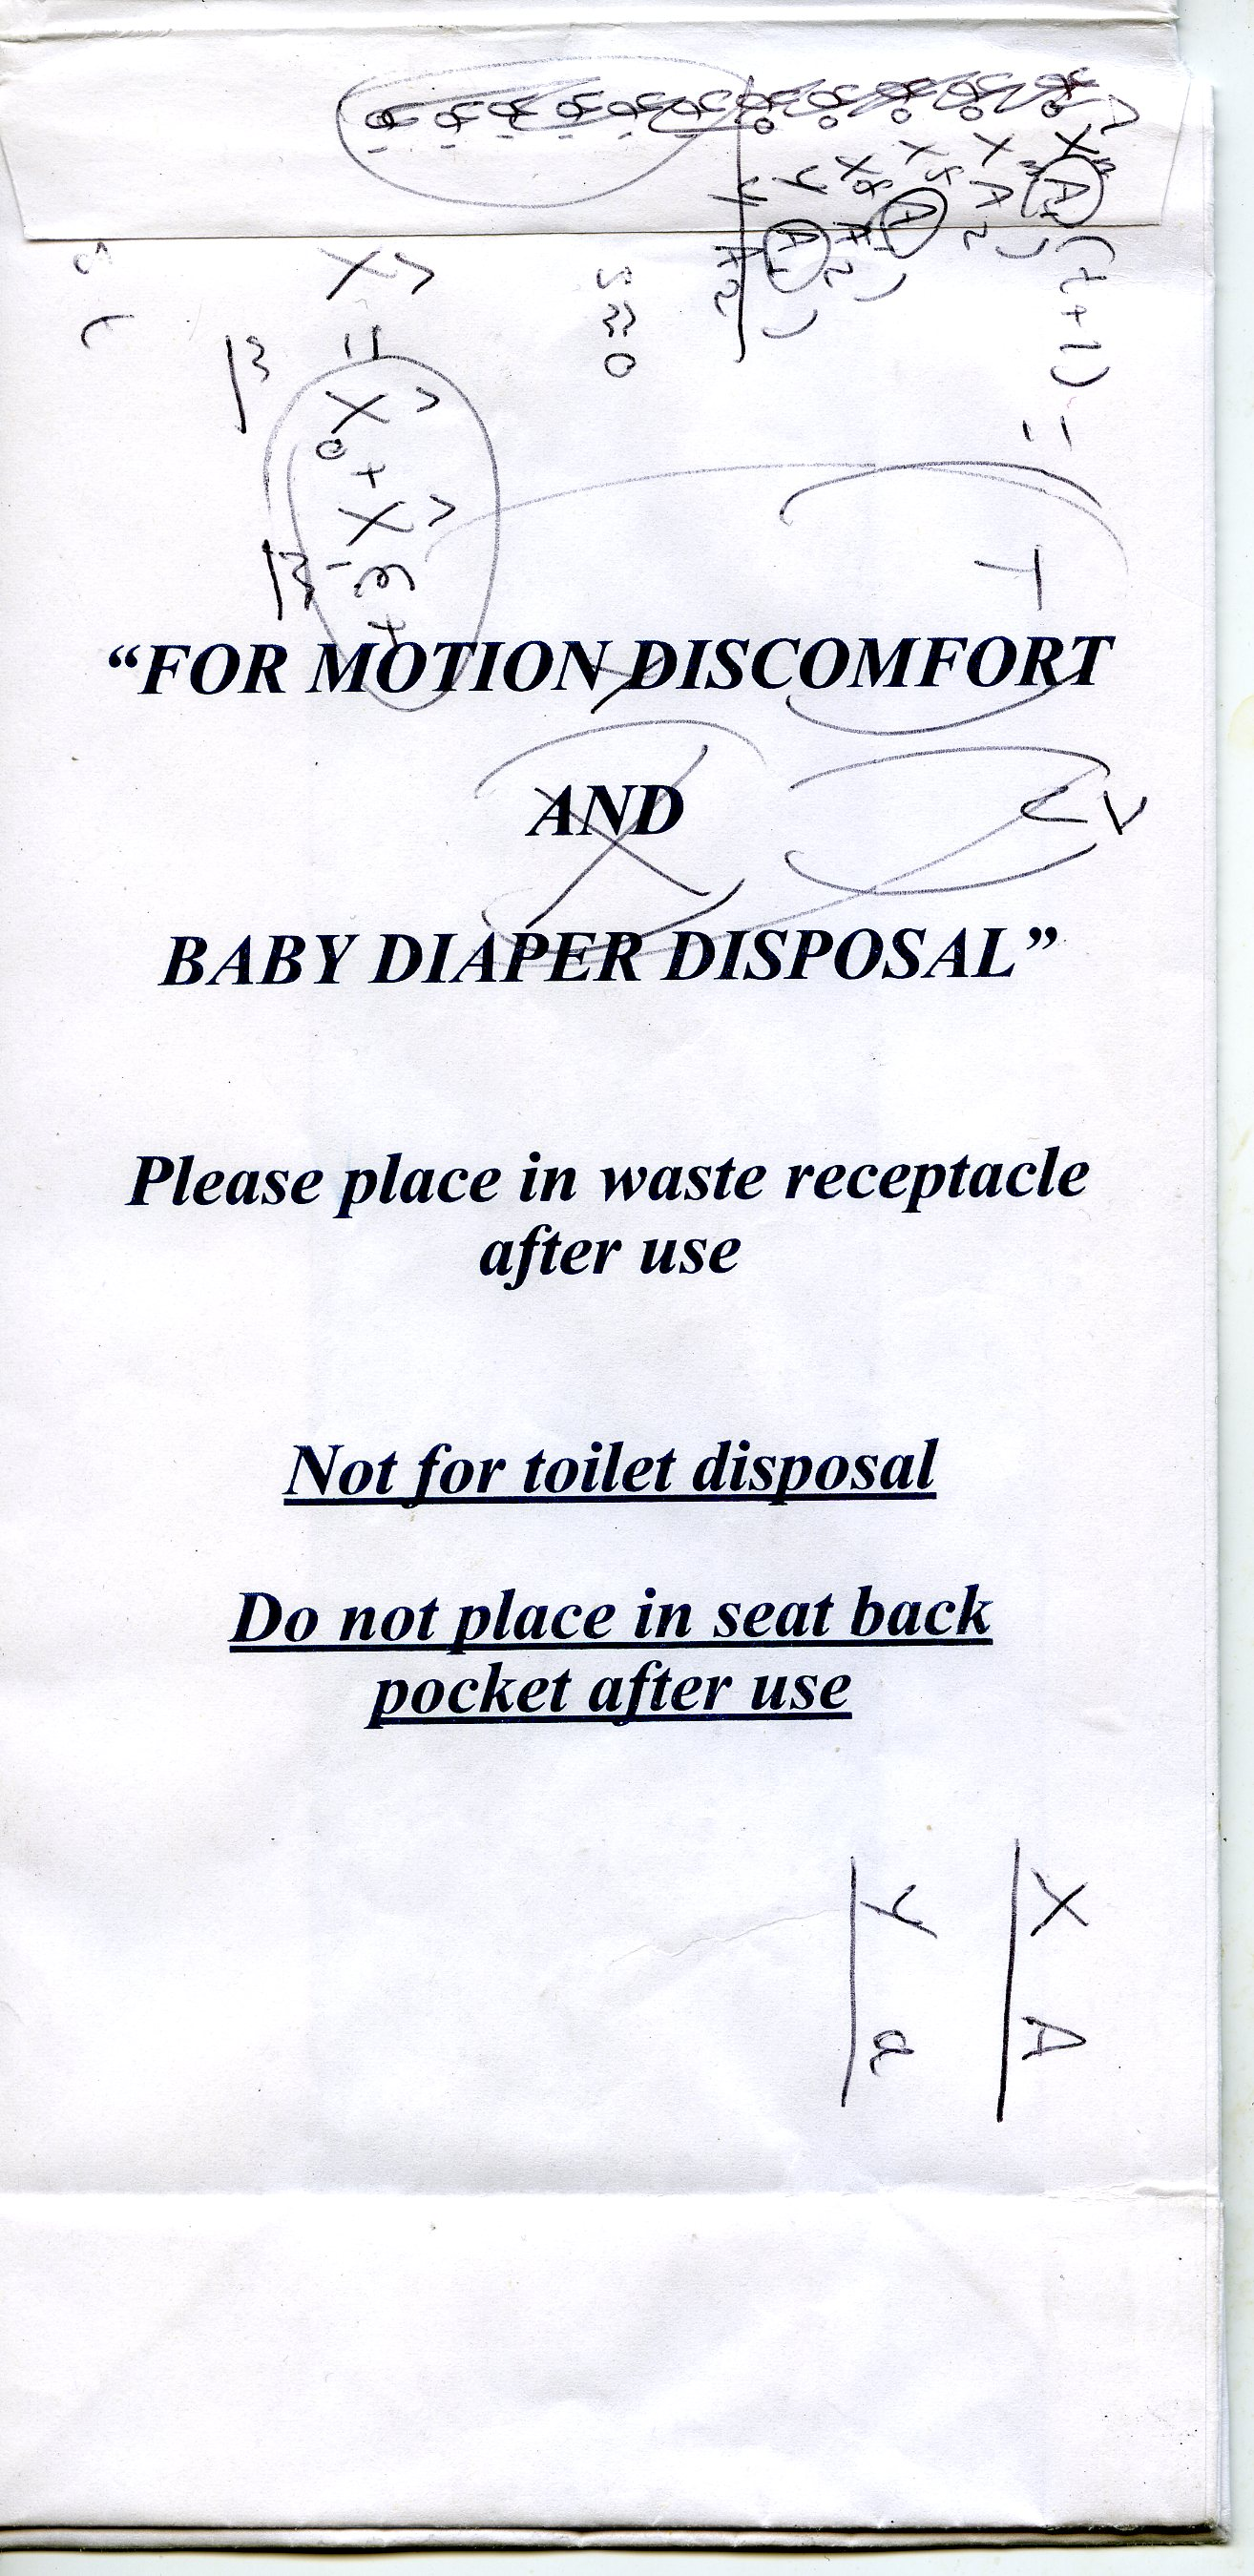
\includegraphics[width=0.4\linewidth, angle=90]{IMAGES/BarfBag2}
%	    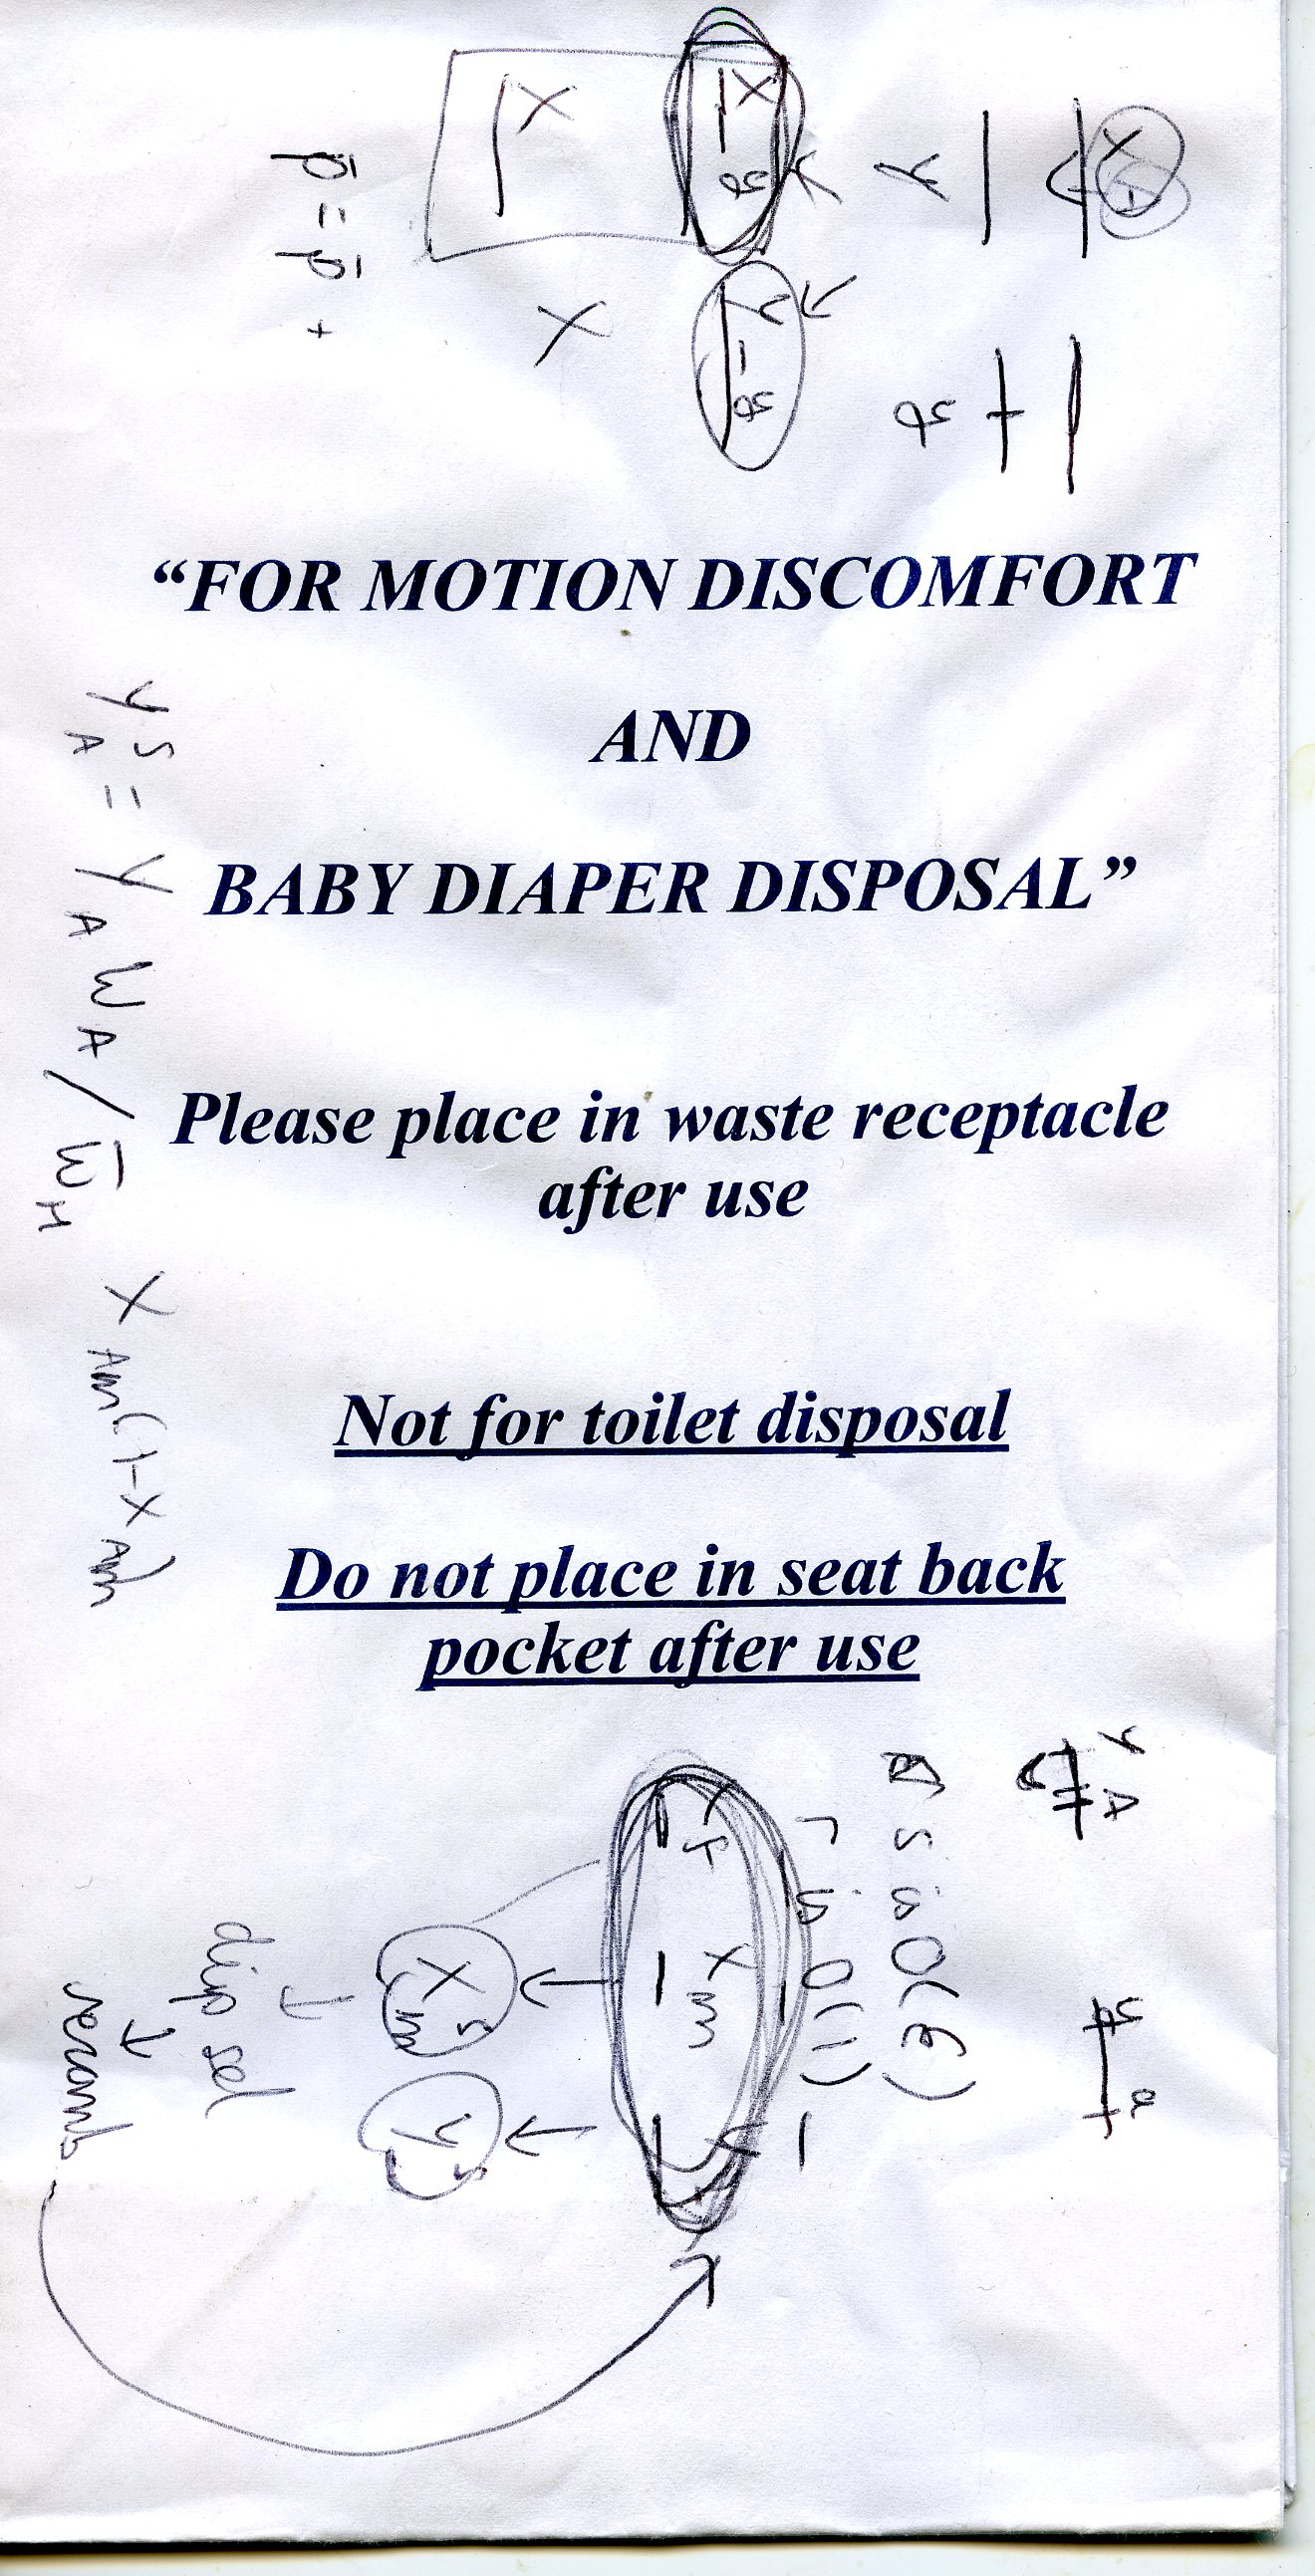
\includegraphics[width=0.4\linewidth, angle=0]{IMAGES/BarfBag1}
%	    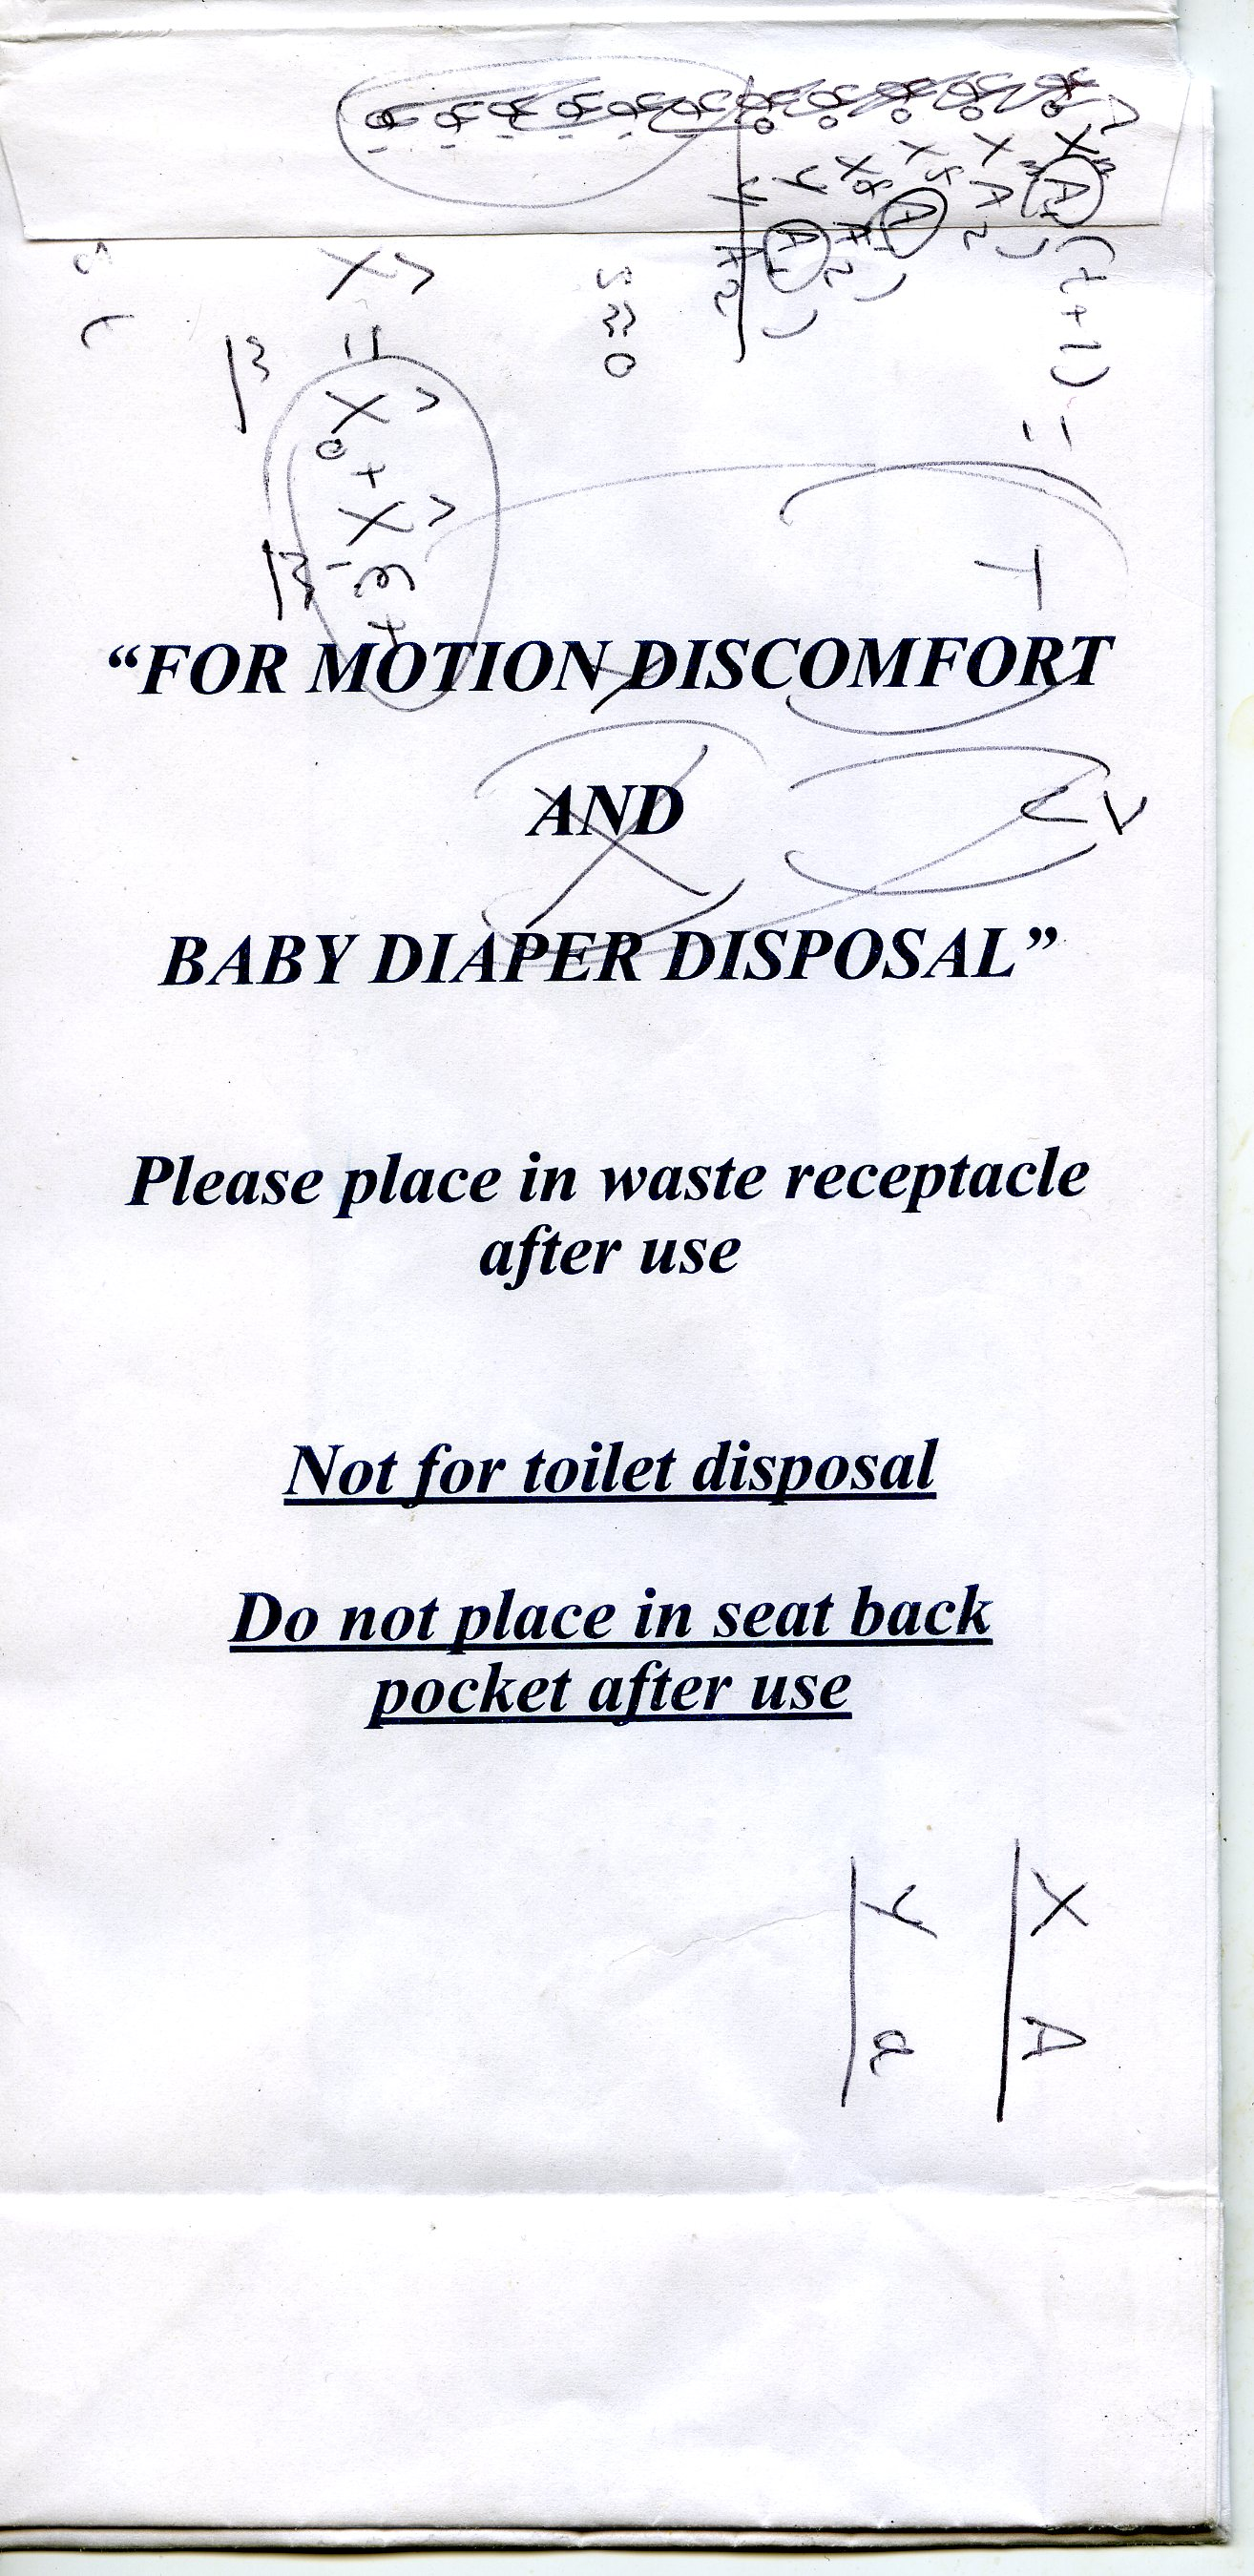
\includegraphics[width=0.4\linewidth, angle=0]{IMAGES/BarfBag2}
	 };
      }  
%      \visible<2->{
%         \node[anchor = south east] at (current page.south east) {
%	    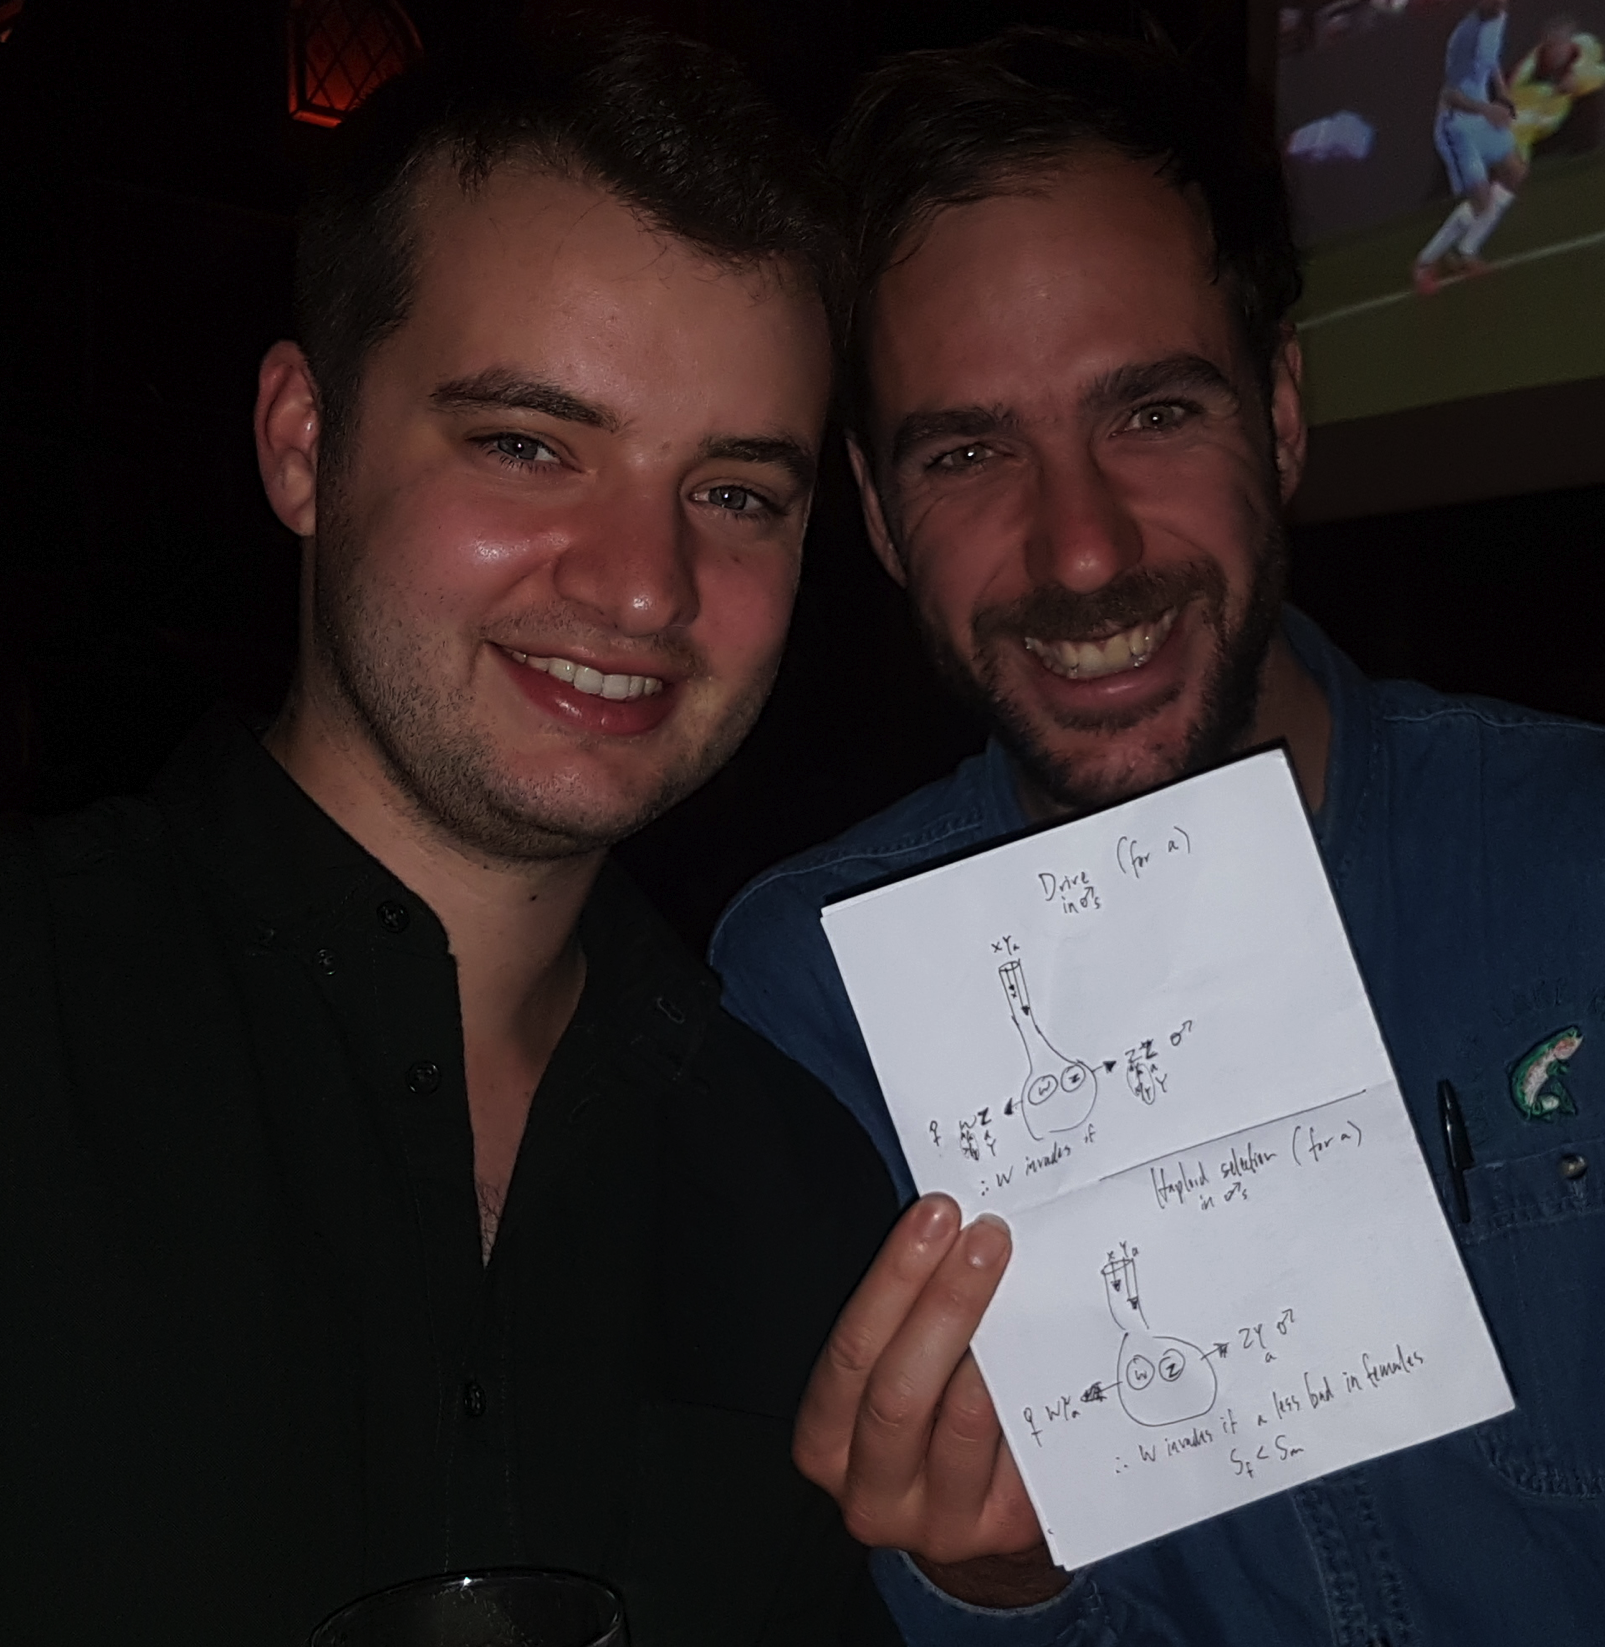
\includegraphics[width=0.3\linewidth]{IMAGES/LondonBar}
%	};
%      }
%infinite popn, random mating, non-overlapping generations
%3 loci (selected, ancestral, dominant novel), 2 alleles at each
      \visible<2>{
         \draw[thick, red] (8.5,-1) circle [radius=1.25, thick];
      } 
      \visible<3->{
         \draw[thick] (8.5,-1) circle [radius=1.25, thick];
      } 
      \visible<2->{
         %chromosomal order (move coordinate C and position of locus A only)  
         \coordinate (C) at (7.5,-0.9);
         \coordinate (A) at ($(C)+(0.5,0)$); 
         \draw[thick] (C) -- ($(C)+(2,-0.1)$);
         \draw[thick] ($(A)+(0,-0.05)$) -- ($(A)+(0,0.05)$) node[above] {}; %{$\textcolor{black}{Y}$};
         \draw[thick] ($(C)+(1,-0.05)$) -- ($(C)+(1,0.05)$) node[above] {}; %{$\textcolor{red}{A}$};
         \draw[thick] ($(C)+(1.5,-0.15)$) -- ($(C)+(1.5,-0.05)$) node[above, yshift=-3] {$\textcolor{blue}{Z}$};  
         %chromosomal order (move coordinate C and position of locus A only)  
         \coordinate (C) at (7.5,-1.48);
         \coordinate (A) at ($(C)+(0.5,0)$); 
         \draw[thick] (C) -- ($(C)+(2,0)$);
         \draw[thick] ($(A)+(0,-0.05)$) -- ($(A)+(0,0.05)$) node[above] {}; %{$\textcolor{black}{Y}$};
         \draw[thick] ($(C)+(1,-0.05)$) -- ($(C)+(1,0.05)$) node[above] {}; %{$\textcolor{red}{A}$};
         \draw[thick] ($(C)+(1.5,-0.05)$) -- ($(C)+(1.5,0.05)$) node[above, yshift=-3] {$\textcolor{blue}{W}$};  
         \node[] at (8.5, -2.5) {
	    3 bi-allelic loci
	};
      } 
      \visible<3>{
         \node[red] at (8.5, -4) {
	    infinite population 
	};
      } 
      \visible<4->{
         \node[] at (8.5, -4) {
	    infinite population 
	};
      } 
      \visible<4>{
         \draw[thick, red] (2.2,3) circle [radius=1, thick];
      } 
      \visible<5->{
         \draw[thick] (2.2,3) circle [radius=1, thick];
      } 
      \visible<4->{
         \node[] at (0, 3) {
	    diploid sel$^n$
	};
       \path[->,thick] (0.15,2.7) edge (0.15,2.3);  
       \node[] at (0, 2) {
	    segregation
	};
       \path[->,thick] (0.15,1.7) edge (0.15,1.3);  
       \node[] at (0, 1) {
	    haploid sel$^n$
	};
       \path[->,thick] (0.15,0.7) edge (0.15,0.3);  
       \node[] at (0.25, 0) {
	    random mating
	};   
       \path[->,thick] (0.15,-0.3) edge (0.15,-0.7);  
   } 
      %recursion equations, stability analyses, numerical simulations
      \visible<5>{
         \draw[thick, red] (2,-1.25) circle [radius=1, thick];
      } 
      \visible<6->{
         \draw[thick] (2,-1.25) circle [radius=1, thick];
      } 
      \visible<5->{
         \node[anchor = west, text width = 2.5cm, yshift = -2cm, xshift=-0.25cm] at (current page.west) {
	    \begin{enumerate} \item recursion equations \end{enumerate}
	};
%         \path[->,thick] (eqns) edge (7.3,2.75);	
      }
      \visible<6>{
         \draw[thick, red] (2.75,-3) circle [radius=0.75, thick];
      } 
      \visible<7->{
         \draw[thick] (2.75,-3) circle [radius=0.75, thick];
      } 
      \visible<6->{
%         \draw[thick] (2.75,-3) circle [radius=0.75, thick];
         \node[anchor = west, text width = 3cm, yshift = -3.5cm, xshift=0cm] at (current page.west) {
	    \begin{enumerate} \setcounter{enumi}{1} \item resident equilibrium \end{enumerate}
	};
%         \path[->,thick] (eqns) edge (7.3,2.75);	
      }
      \visible<7>{
         \draw[thick, red] (3.5,-1) circle [radius=0.75, thick];
      } 
      \visible<8->{
         \draw[thick] (3.5,-1) circle [radius=0.75, thick];
      } 
      \visible<7->{
%         \draw[thick] (3.5,-1) circle [radius=0.75, thick];
         \node[anchor = west, text width = 2.5cm, yshift = 0cm, xshift=4.5cm] at (current page.west) {
	    \begin{enumerate} \setcounter{enumi}{2} \item invasion analysis \end{enumerate}
	};
%         \path[->,thick] (8.5,-3) edge (3.5,-1);	
      }   
      \visible<8>{
         \draw[thick, red] (7.75,2.75) circle [radius=0.75, thick];
      } 
%      \visible<9->{
%         \draw[thick] (7.75,2.75) circle [radius=0.75, thick];
%      } 
      \visible<8->{
%         \draw[thick] (7.75,2.75) circle [radius=0.75, thick];
         \node[anchor = east, text width = 3cm, yshift = 2.5cm, xshift=10] at (current page.east) {
	    \begin{enumerate} \setcounter{enumi}{3} \item approximate leading eigenvalue \end{enumerate}
	};
%         \path[->,thick] (8.5,-3) edge (3.5,-1);	
      }   
   \end{tikzpicture}
\end{frame}	
%%%%%%%%%%%%%%%%%%%%%%%%%%%%%%%%%%%%%%%%%%%%%%%%%

%%%%%%%%%%%%%%%%%%%%%%%%%%%%%%%%%%%%%%%%%%%%%%%%%
\begin{frame}
   \begin{tikzpicture}[overlay, remember picture]
         \node[anchor = center] at (current page.center) {
           \huge 2 results
	};
   \end{tikzpicture}
\end{frame}
%%%%%%%%%%%%%%%%%%%%%%%%%%%%%%%%%%%%%%%%%%%%%%%%%

%%%%%%%%%%%%%%%%%%%%%%%%%%%%%%%%%%%%%%%%%%%%%%%%%
\begin{frame}
%\frametitle{Result 1} %: Turnover can \textcolor{red}{\textit{create}} sex-ratio bias} %ploidally antagonistic selection
   \begin{tikzpicture}[overlay, remember picture]
      \visible<1->{
         \node[anchor = center, text width = 1.2\linewidth, yshift=80, xshift=5] at (current page.center) {
            \Large \underline{Scenario}: Drive for $\textcolor{red}{a}$ in males opposes selection for $\textcolor{red}{A}$ in diploids
        };
      }   
      \visible<1-2>{
        \node[] at (7,-0.25) {
           \huge $XY \rightarrow \textcolor{blue}{ZW}$?
        };
      }   
%        \node[] at (9,3) {
%           ZW $\rightarrow$ XY
%        };
      \visible<1->{
         %chromosomal order (move coordinate C and position of locus A only)  
         \coordinate (C) at (5.6,0.5);
         \coordinate (A) at ($(C)+(1.7,0)$); 
         \draw[thick] (C) -- ($(C)+(1,0)$);
         \draw[thick] ($(C)+(1.5,0)$) -- ($(C)+(2.5,0)$);
         \draw[thick] ($(A)+(0,-0.05)$) -- ($(A)+(0,0.05)$) node[above] {$\textcolor{red}{A}$};
         \draw[thick] ($(C)+(0.5,-0.05)$) -- ($(C)+(0.5,0.05)$) node[above] {$\textcolor{black}{Y}$};
         \draw[thick] ($(C)+(2,-0.05)$) -- ($(C)+(2,0.05)$) node[above] {$\textcolor{blue}{W}$};  
%        \node[] at (6,3) {
%           \textcolor{gray}{$r=0.5 \rightarrow R=0.05$}
%        };        
%        \node[text width=4cm] at (3.5,3) {
%           $\begin{aligned}
%           XY &\rightarrow ZW\\
%           r=0.5 &\rightarrow R=0.05
%           \end{aligned}$
%        };
%        \node[] at (8.5,3) {
%           $\begin{aligned}
%           ZW &\rightarrow XY\\
%           r=0.5 &\rightarrow R=0.05
%           \end{aligned}$
%        };
      }   
      \visible<2>{
        \node[text width = \linewidth] at (5,-2) {
           \Large no sex-ratio bias\\
           \Large no antagonism between diploid sexes
        };
      }   
      \visible<3->{
         \node[anchor = south, text width = 0.9\linewidth, yshift=0] at (current page.south) {
%%	    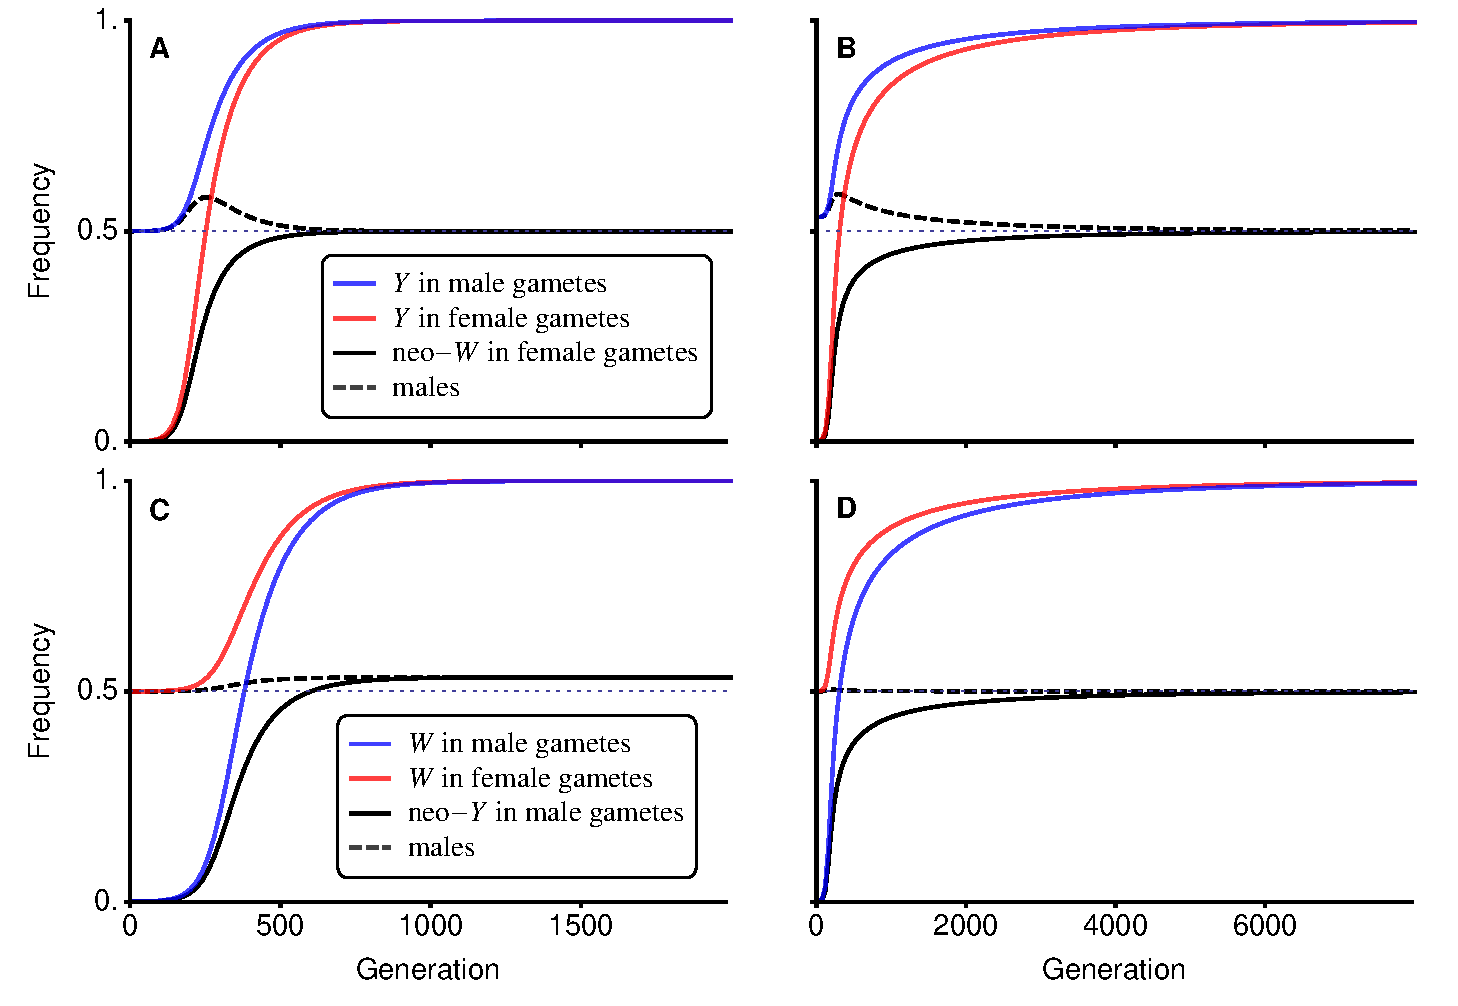
\includegraphics[width=\linewidth, angle=0]{../Plots/Combination_Turnover}
%	    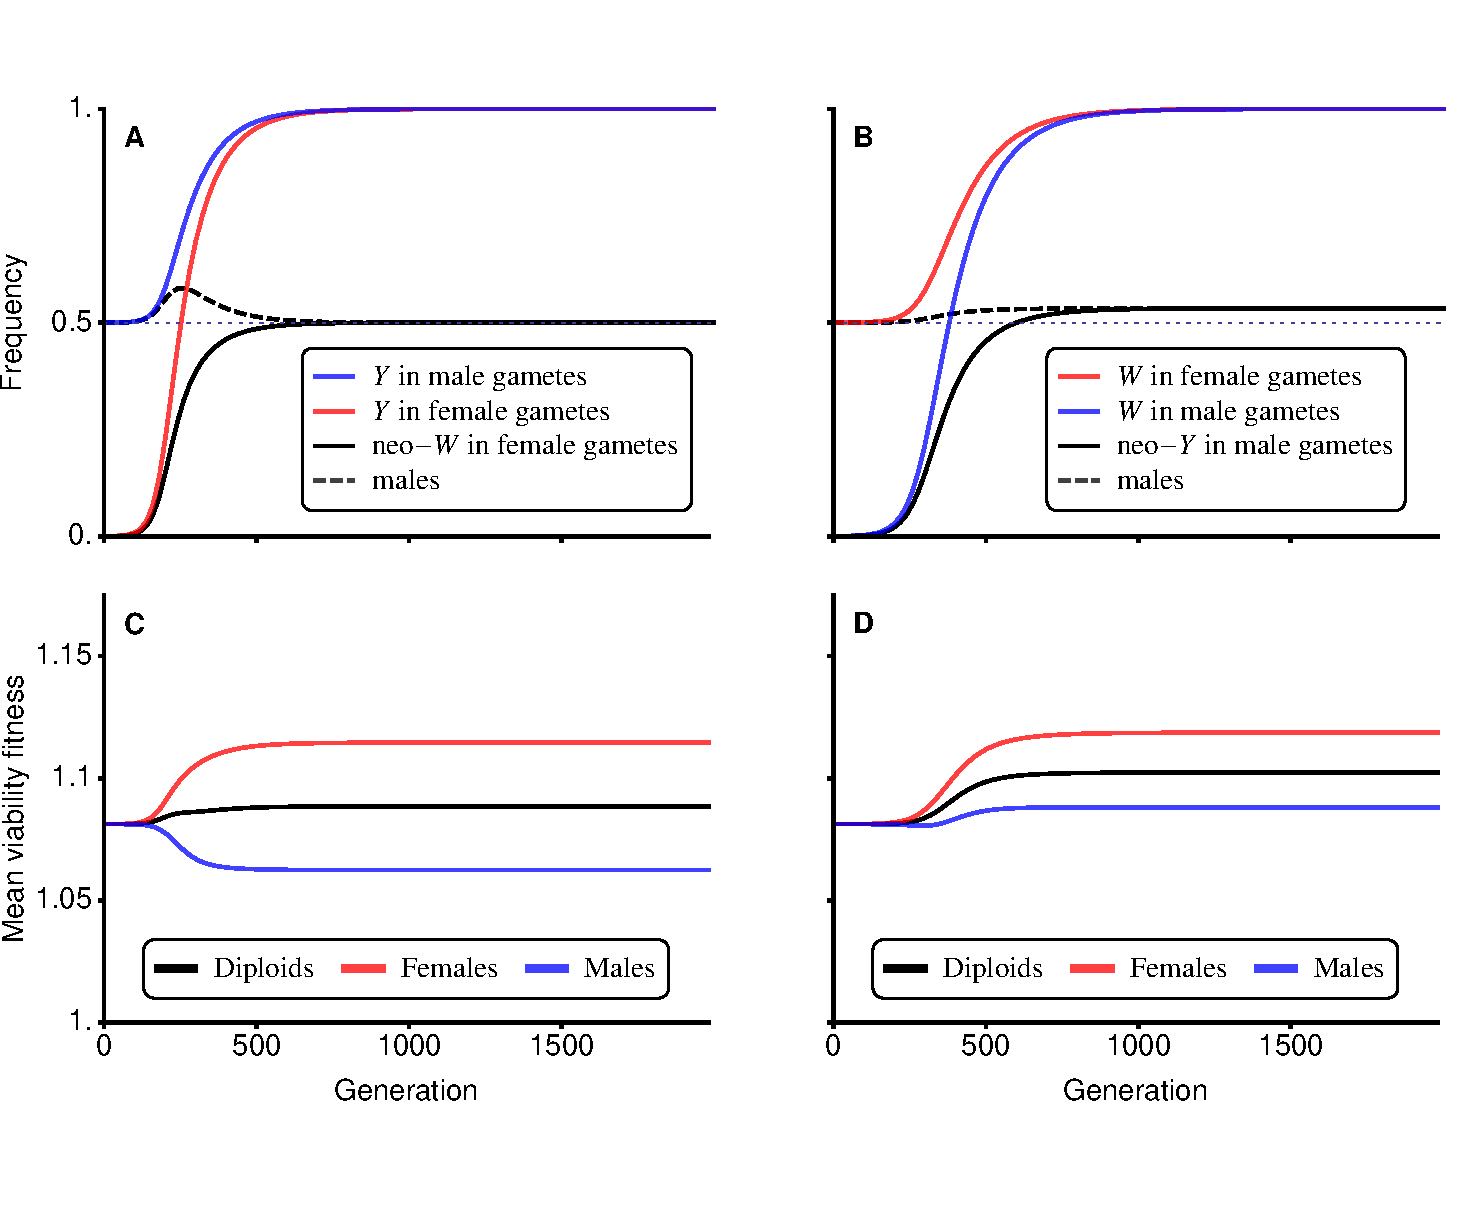
\includegraphics[width=\linewidth, angle=0]{../Plots/Combination_TurnoverMeanFit_Tighter}
	    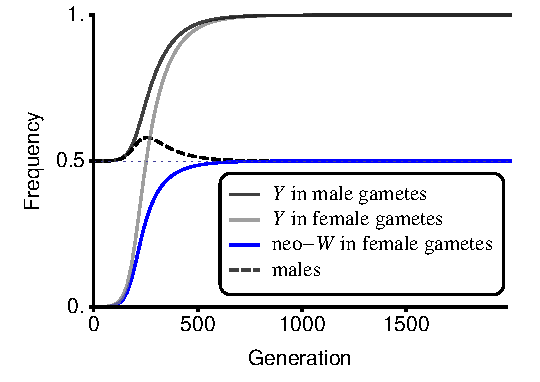
\includegraphics[width=\linewidth, angle=0]{../Plots/Combination_Turnover_Evo}
	 };
%       \node[rotate = 90] at (-0.5,-2.5) {
%           ZW $\rightarrow$ XY
%        };
      }   
      \visible<3->{
        \node[] at (7,-0.25) {
           \huge $XY \rightarrow \textcolor{blue}{ZW}$!
        };
      }   
      \visible<4->{
         \draw[red,very thick] (3.5,-1) circle [radius=1];
         \node[anchor = center, yshift=110, xshift=0] at (current page.center) {
%            \Large \textcolor{blue}{Result 1}: Turnover can \textcolor{red}{\textit{create}} sex-ratio bias
         \begin{tcolorbox}[colback=blue!5!white,colframe=blue!75!black]
	   \Large \textcolor{blue}{Result 1}: Turnover \textcolor{red}{\textit{regardless}} of sex-ratio bias
	\end{tcolorbox}	
        };
      }   
   \end{tikzpicture}
\end{frame}
%%%%%%%%%%%%%%%%%%%%%%%%%%%%%%%%%%%%%%%%%%%%%%%%%

%%%%%%%%%%%%%%%%%%%%%%%%%%%%%%%%%%%%%%%%%%%%%%%%%
%\begin{frame}
%   \begin{tikzpicture}[overlay, remember picture]
%      \visible<1->{
%         \node[anchor = center, text width = \linewidth] at (current page.center) {
%	 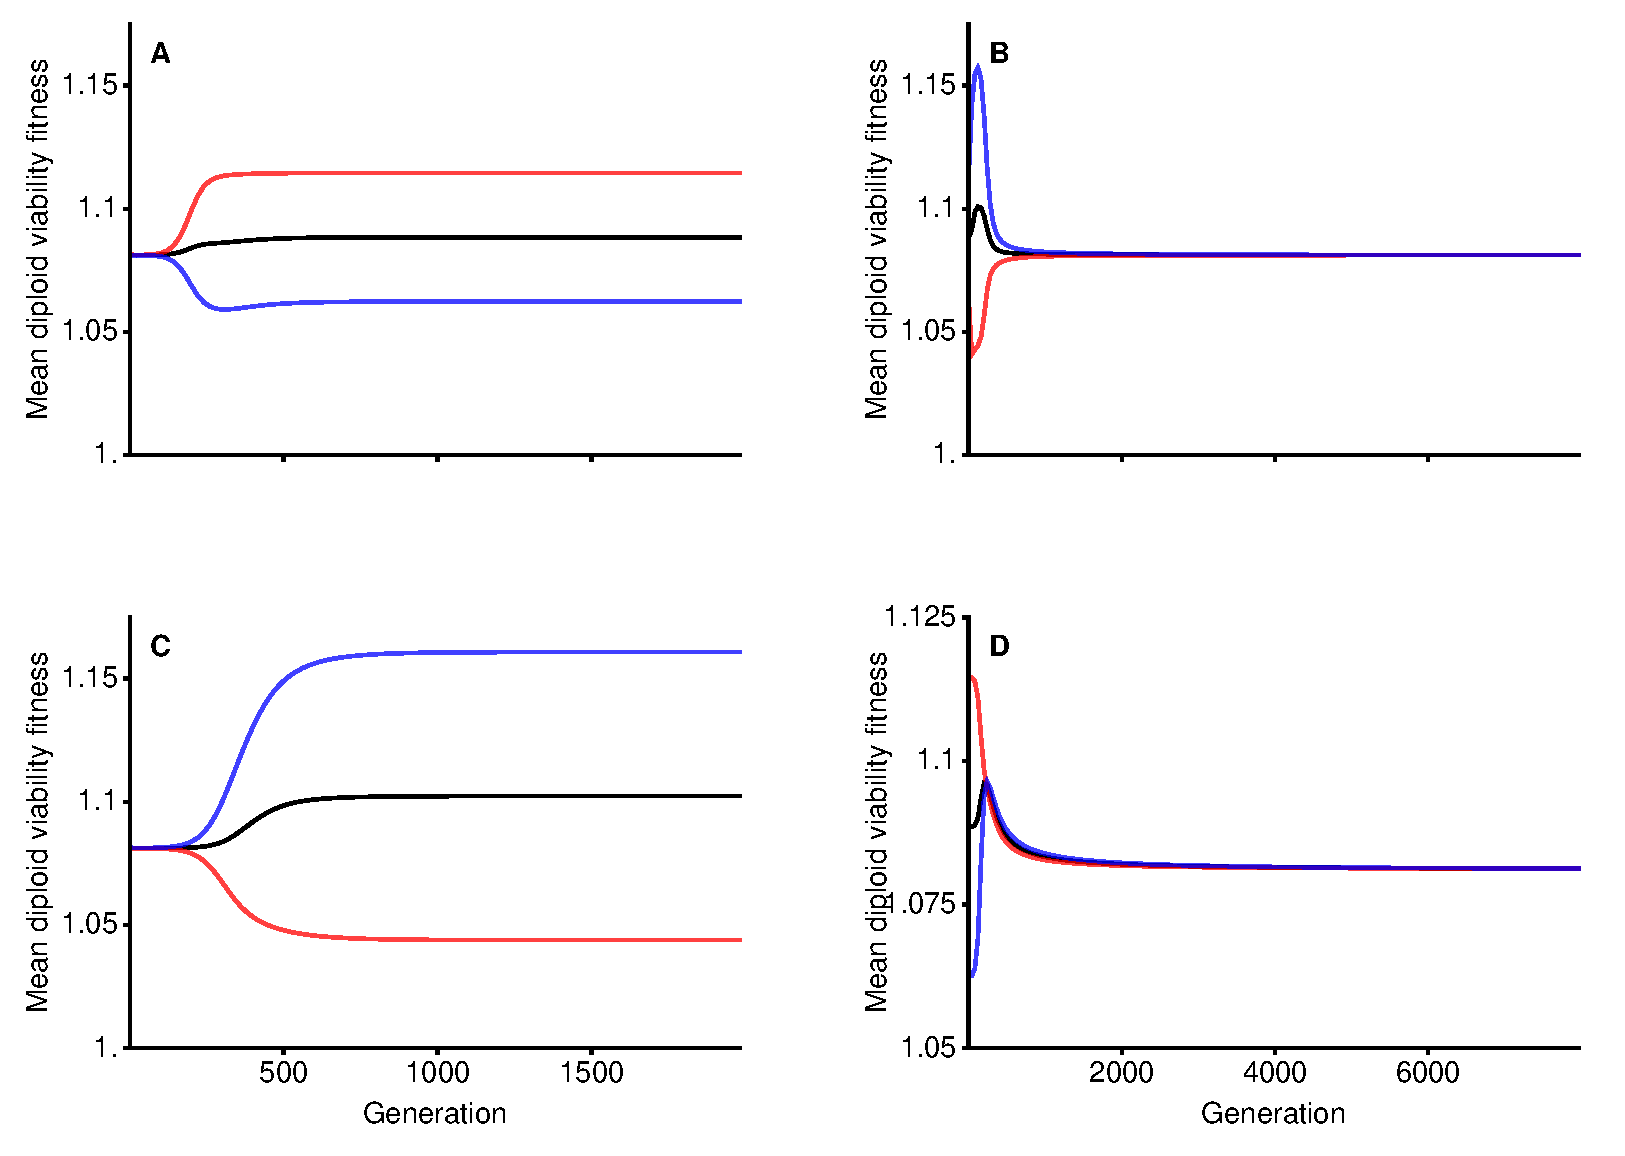
\includegraphics[width=\linewidth, angle=0]{../Plots/Combination_MeanFit}
%	 };
%      } 
%   \end{tikzpicture}
%\end{frame}
%%%%%%%%%%%%%%%%%%%%%%%%%%%%%%%%%%%%%%%%%%%%%%%%%

%%%%%%%%%%%%%%%%%%%%%%%%%%%%%%%%%%%%%%%%%%%%%%%%%
\begin{frame}
   \begin{tikzpicture}[overlay, remember picture]
      \visible<1->{
         \node[anchor = center, text width = 1.2\linewidth, yshift=80, xshift=5] at (current page.center) {
            \Large \underline{Scenario}: Drive for $\textcolor{red}{a}$ in males opposes selection for $\textcolor{red}{A}$ in diploids
        };
      }   
      \visible<2-7>{
         \node[anchor = south, text width = 0.9\linewidth, yshift=0] at (current page.south) {
	    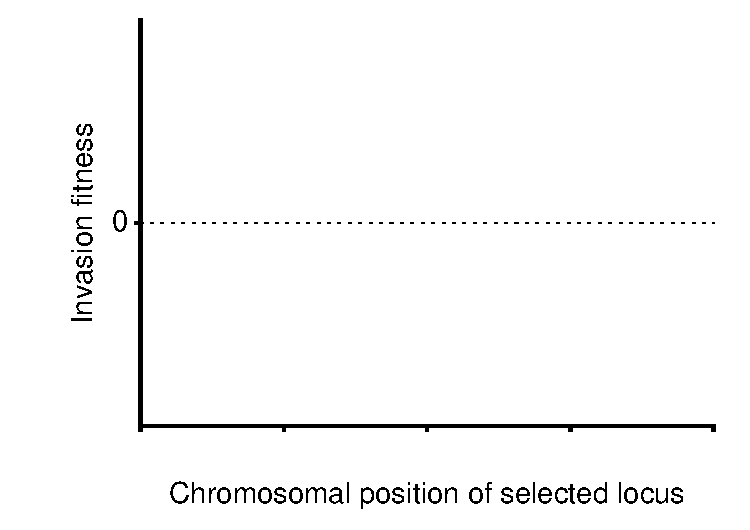
\includegraphics[width=\linewidth, angle=0]{../Plots/PositionPlotB_Evo_Empty}
	 };
      }   
%   \visible<1-2>{
%        \node[] at (7,-0.25) {
%           \huge $XY \rightarrow \textcolor{blue}{ZW}$?
%        };
%      }    
      \visible<8->{
         \node[anchor = south, text width = 0.9\linewidth, yshift=0] at (current page.south) {
	    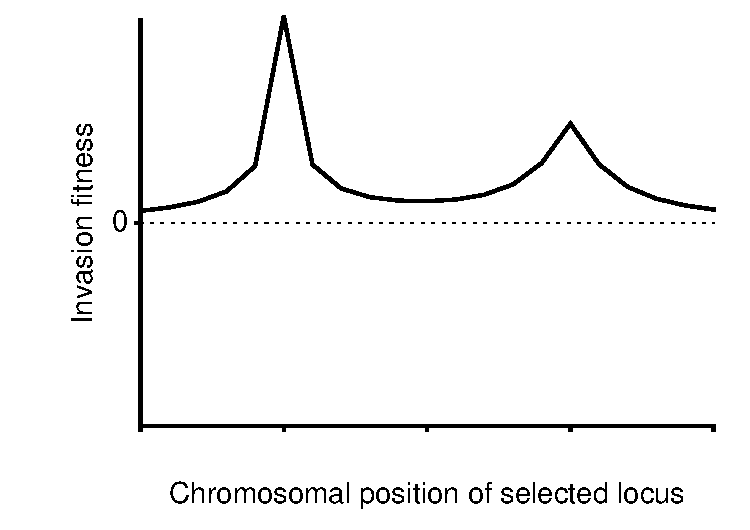
\includegraphics[width=\linewidth, angle=0]{../Plots/PositionPlotB_Evo}
	 };
      }   
      \visible<2->{
         \node[anchor = center, xshift= 125, yshift = -120] at (current page.center) {
            ($\textcolor{red}{A}$)
         };         
      }    
      \visible<2->{
         \node[anchor=center] at (7.9,-4.25)  {
            $\textcolor{blue}{W}$
         };                 
          \node[anchor=center] at (4.2,-4.25)  {
             $\textcolor{black}{Y}$
          };         
      }    
      \visible<5->{
         \draw [decorate,decoration={brace,mirror,amplitude=10pt,raise=0pt},yshift=0pt,thick]
            (2.5,-2.75) -- (6,-2.75) node [black,midway,yshift=-20] {
               looser linkage
            };   
         \draw [decorate,decoration={brace,mirror,amplitude=10pt,raise=0pt},yshift=0pt,thick]
            (6.25,-2.75) -- (9.75,-2.75) node [black,midway,yshift=-20] {
               tighter linkage
            };   
      }    
      \visible<3->{
         %chromosomal order (move coordinate C and position of locus A only)  
         \coordinate (C) at (2.75,-2.5);
         \coordinate (A) at ($(C)+(1,0)$); 
         \draw[thick] (C) -- ($(C)+(3,0)$);
         \draw[thick] ($(A)+(0,-0.05)$) -- ($(A)+(0,0.05)$) node[above] {$\textcolor{red}{A}$};
         \draw[thick] ($(C)+(0.5,-0.05)$) -- ($(C)+(0.5,0.05)$) node[above] {$\textcolor{black}{Y}$};
         \draw[thick] ($(C)+(2,-0.05)$) -- ($(C)+(2,0.05)$) node[above] {$\textcolor{blue}{W}$};  
         %chromosomal order (move coordinate C and position of locus A only)  
         \coordinate (C) at (6.5,-2.5);
         \coordinate (A) at ($(C)+(1.5,0)$); 
         \draw[thick] (C) -- ($(C)+(3,0)$);
         \draw[thick] ($(A)+(0,-0.05)$) -- ($(A)+(0,0.05)$) node[above] {$\textcolor{red}{A}$};
         \draw[thick] ($(C)+(0.5,-0.05)$) -- ($(C)+(0.5,0.05)$) node[above] {$\textcolor{black}{Y}$};
         \draw[thick] ($(C)+(2,-0.05)$) -- ($(C)+(2,0.05)$) node[above] {$\textcolor{blue}{W}$};  
      }    
      \visible<4->{
         \draw [decorate,decoration={brace,amplitude=10pt,raise=4pt},yshift=0pt,thick]
            (1,-1.25) -- (1,1.25) node [black,midway,xshift=-20,rotate=90] {
               neo-$\textcolor{blue}{W}$ invades
            };   
      }  
%%   \visible<3->{
%%        \node[] at (7,-0.25) {
%%           \huge $XY \rightarrow \textcolor{blue}{ZW}$!
%%        };
%%      }   
      \visible<6-7>{
         \node[] at (4,0) {
	   \huge ?
        };
         \node[] at (8,0) {
	   \huge \checkmark
        };
      }   
      \visible<9->{
         \draw[red,very thick] (4.25,0) circle [radius=1.5];
         \node[anchor = center, yshift=110, xshift=0] at (current page.center) {
            \begin{tcolorbox}[colback=blue!5!white,colframe=blue!75!black]
	      \Large \textcolor{blue}{Result 2}: Turnover despite \textcolor{red}{\textit{looser}} sex-linkage
	   \end{tcolorbox}	
        };
      }   
      \visible<7->{
         \node[anchor = center, yshift = 30, xshift=130] at (current page.center) {
            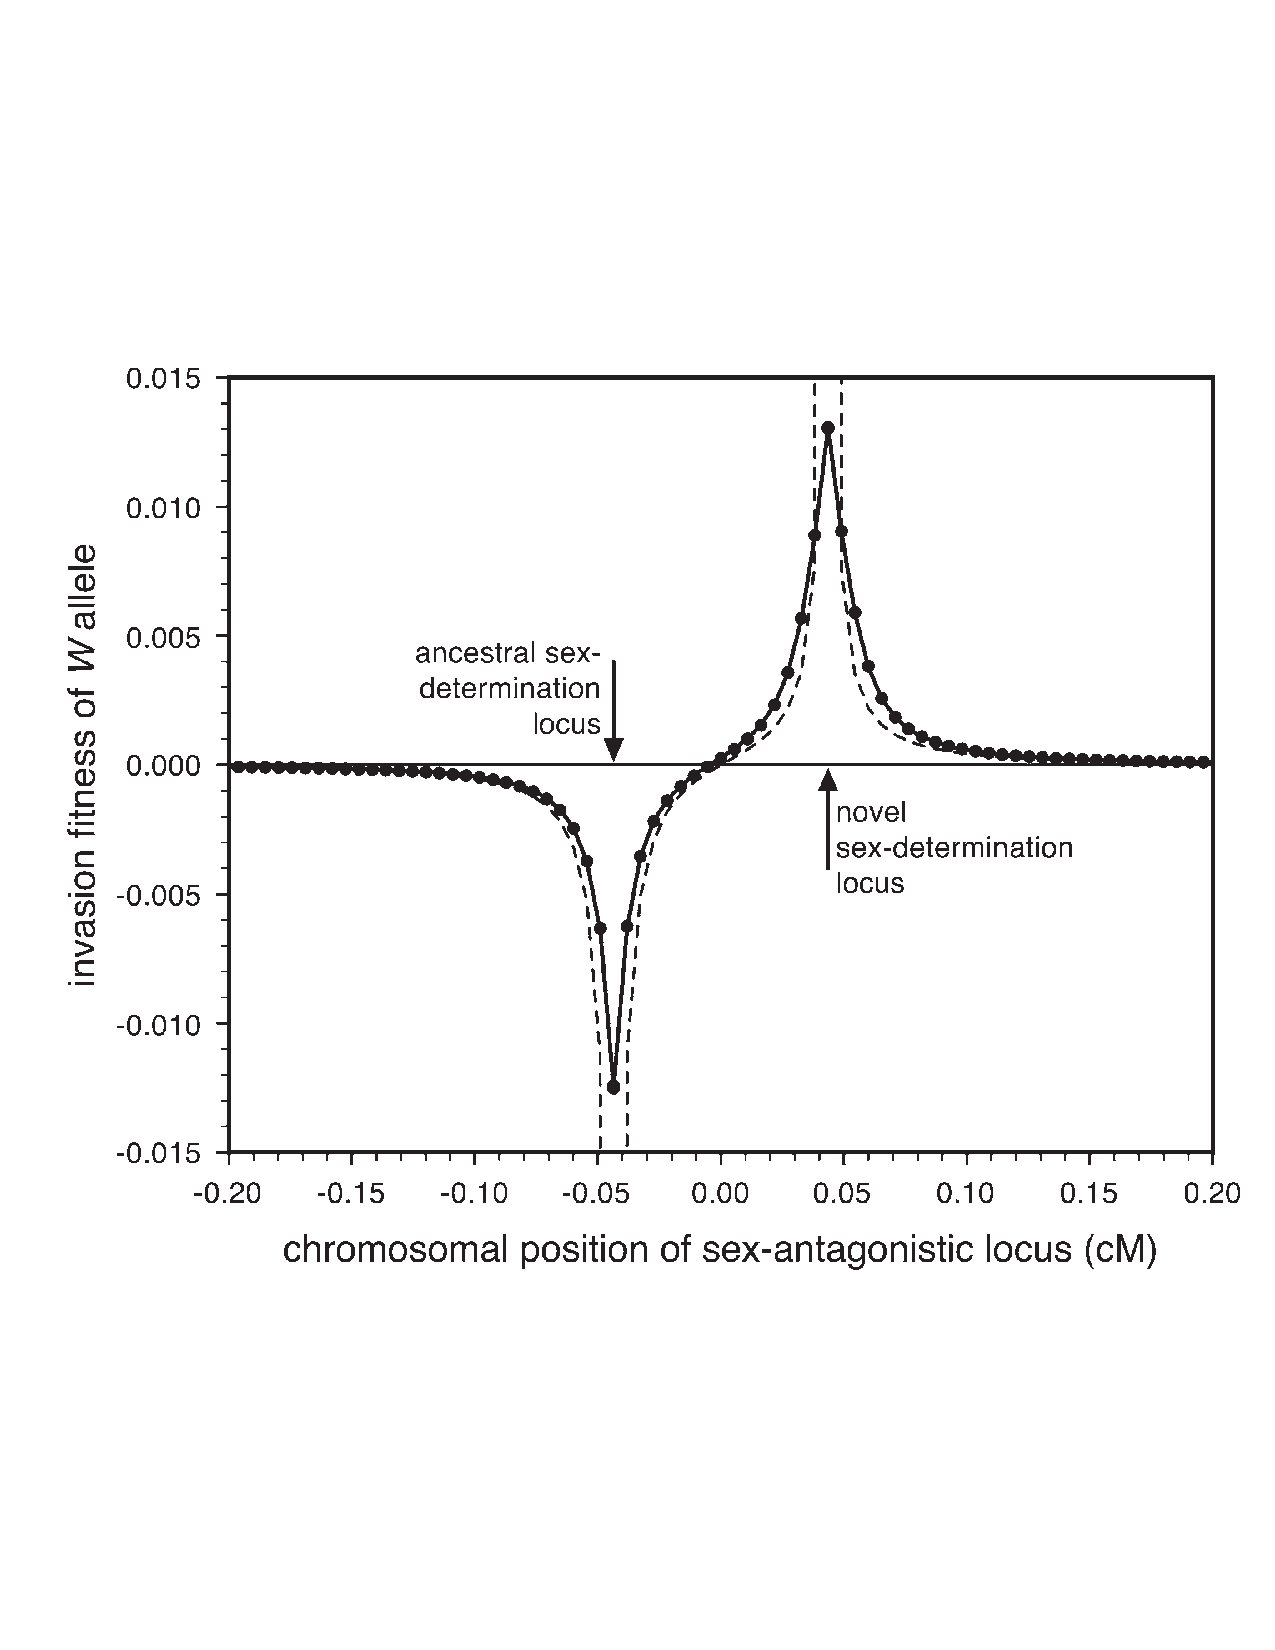
\includegraphics[width=0.3\linewidth, angle=0]{IMAGES/vanDoornKirkpatrick2010Fig2}
        };
      }   
   \end{tikzpicture}
\end{frame}
%%%%%%%%%%%%%%%%%%%%%%%%%%%%%%%%%%%%%%%%%%%%%%%%%

%%%%%%%%%%%%%%%%%%%%%%%%%%%%%%%%%%%%%%%%%%%%%%%%%
%\begin{frame}
%\frametitle{Result 2: Turnover despite \textcolor{red}{\textit{looser}} sex-linkage}
%   \begin{tikzpicture}[overlay, remember picture]
%         \node[anchor = south, text width = \linewidth] at (current page.south) {
%	    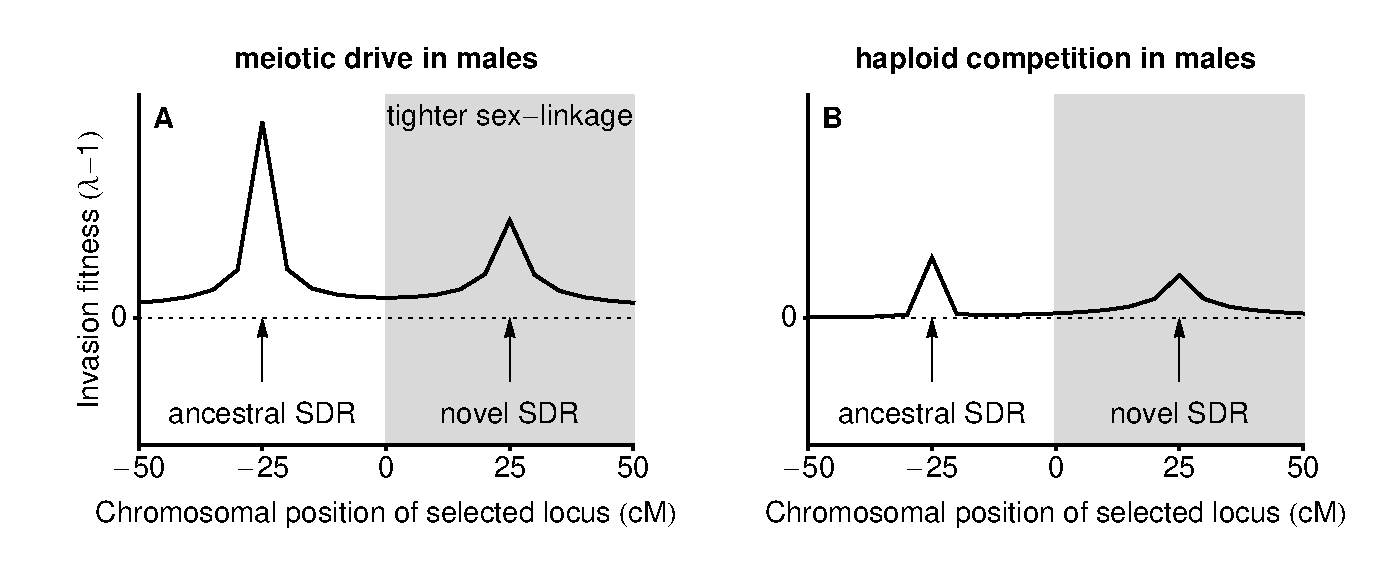
\includegraphics[width=\linewidth, angle=0]{../Plots/PositionPlot}
%	 };
%       \node[anchor=east] at (6,0) {
%           sexually-antagonistic
%        };
%       \node[anchor=east] at (11,0) {
%           drive opposes diploid sel$^n$
%        };
%       \node[anchor=east] at (6,-3.5) {
%           ploidally-antagonsitic
%        };
%       \node[anchor=east] at (6,-1.25) {
%           \textcolor{gray}{(stronger sel$^n$ in females)}
%        };     
%       \node[anchor=east] at (11,-3.5) {
%           ploidally-antagonsitic
%        };   
%       \node[anchor=east] at (11,-1.25) {
%            \textcolor{gray}{(stronger sel$^n$ in males)}
%        };
%       \node[anchor=center] at (7.3,3.4)  {
%          \textcolor{gray}{ancestral SD}
%        };
%       \path[->,thick,gray] (7.3,3.2) edge (7.3,2.75);           
%       \node[anchor=center] at (9.4,3.4) {
%          \textcolor{gray}{novel SD}
%        };                       
%       \path[->,thick,gray] (9.4,3.2) edge (9.4,2.75);  
%   \end{tikzpicture}
%\end{frame}
%%%%%%%%%%%%%%%%%%%%%%%%%%%%%%%%%%%%%%%%%%%%%%%%%

%%%%%%%%%%%%%%%%%%%%%%%%%%%%%%%%%%%%%%%%%%%%%%%%%
%\begin{frame}
%\frametitle{Result 2b: Looser linkage evolves despite fitness \textcolor{red}{\textit{decline}}}
%   \begin{tikzpicture}[overlay, remember picture]
%         \node[anchor = south, text width = 0.5\linewidth, yshift=-20] at (current page.south) {
%%	    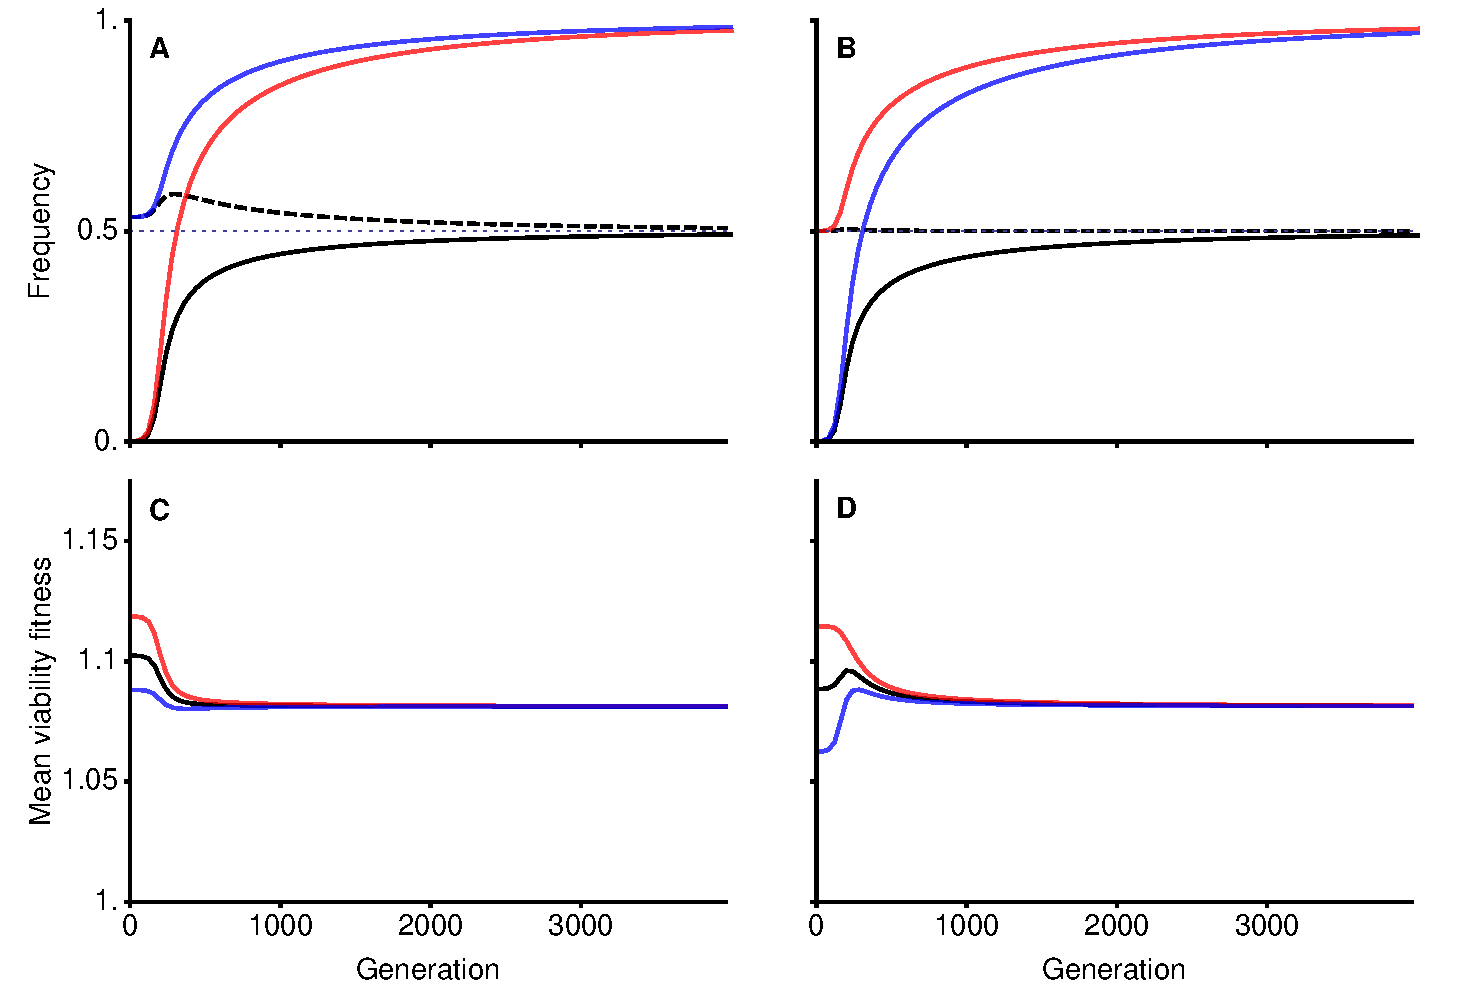
\includegraphics[width=\linewidth, angle=0]{../Plots/Combination_TurnoverMeanFit_Looser}
%	    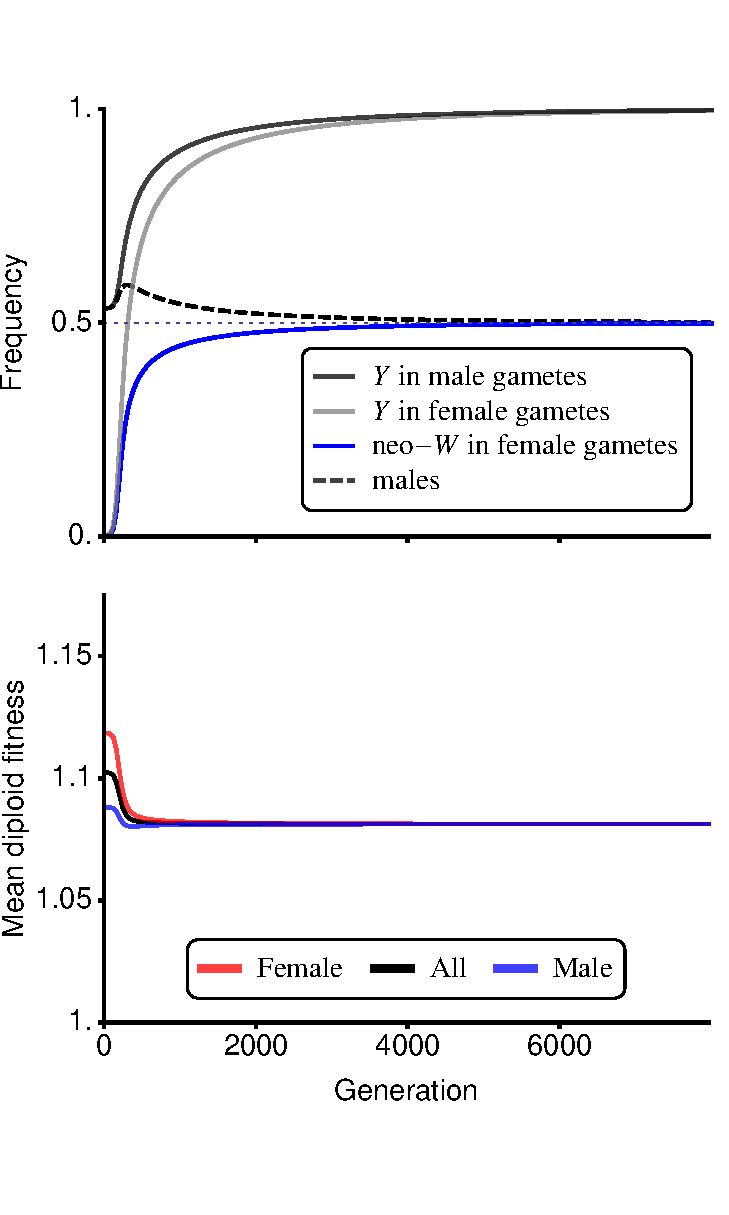
\includegraphics[width=\linewidth, angle=0]{../Plots/Combination_Turnover_Evo2}
%	 };
%%        \node[] at (3,3) {
%%           XY $\rightarrow$ ZW
%%        };
%%        \node[] at (9,3) {
%%           ZW $\rightarrow$ XY
%%        };
%%        \node[] at (6,3) {
%%           \textcolor{gray}{$r=0.05 \rightarrow R=0.5$}
%%        };      
%%       \node[rotate = 90] at (-0.5,-0.75) {
%%          Drive in males opposes selection in diploids
%%        };          
%   \end{tikzpicture}
%\end{frame}
%%%%%%%%%%%%%%%%%%%%%%%%%%%%%%%%%%%%%%%%%%%%%%%%%

%%%%%%%%%%%%%%%%%%%%%%%%%%%%%%%%%%%%%%%%%%%%%%%%%
%\begin{frame}
%\frametitle{Bonus result! Turnover with very tight linkage}
%   \begin{tikzpicture}[overlay, remember picture]
%         \node[anchor = south, xshift=-1cm] at (current page.south) {
%	    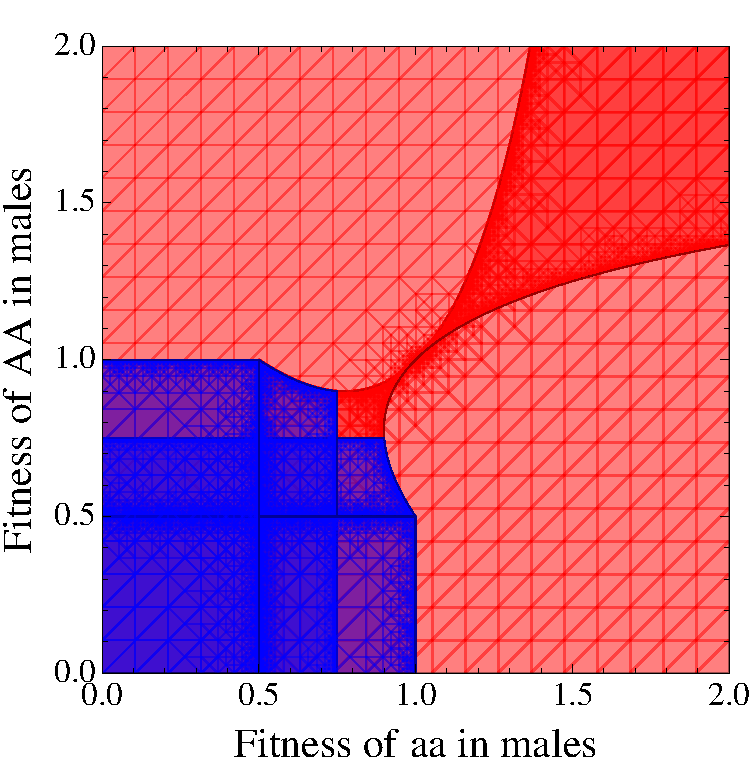
\includegraphics[width=0.75\linewidth, angle=0]{../Plots/regionplot_2b}
%	 };
%       \node[rotate = 90] at (-0.5,-0.75) {
%          Overdominance in diploids, no haploid selection
%        };
%       \node[text width = 3cm] at (10,1) {
%          \textcolor{red}{neo-W invades XY linked to X allele}
%       };
%       \node[text width = 3cm] at (10,-2) {
%          \textcolor{blue}{neo-W invades XY linked to Y allele!}
%       };                              
%   \end{tikzpicture}
%\end{frame}
%%%%%%%%%%%%%%%%%%%%%%%%%%%%%%%%%%%%%%%%%%%%%%%%%

%%%%%%%%%%%%%%%%%%%%%%%%%%%%%%%%%%%%%%%%%%%%%%%%%
\begin{frame}
\frametitle{Summary}
   \begin{tikzpicture}[overlay, remember picture]
      \visible<1->{
         \node[anchor = center, text width = 1.15\linewidth, yshift=50] at (current page.center) {
	    \huge Haploid selection creates new avenues for sex determination turnover
         };                              
      }
      \visible<2->{
         \node[anchor = center, text width = 1.15\linewidth, yshift=-10] at (current page.center) {
            \begin{tcolorbox}[colback=blue!5!white,colframe=blue!75!black]
	      \Large \textcolor{blue}{Result 1}: Turnover \textcolor{red}{\textit{regardless}} of sex-ratio bias
	   \end{tcolorbox}	         
	   };                              
      }
      \visible<3->{
         \node[anchor = center, text width = 1.15\linewidth, yshift=-60] at (current page.center) {
            \begin{tcolorbox}[colback=blue!5!white,colframe=blue!75!black]
	      \Large \textcolor{blue}{Result 2}: Turnover despite \textcolor{red}{\textit{looser}} sex-linkage
	   \end{tcolorbox}	         
	   };                              
      }
      \visible<4->{
         \node[anchor = center, text width = 1.15\linewidth, yshift=-110] at (current page.center) {
	   \huge More turnover in haploid-diploid organisms?         
	   };                              
      }
%      \visible<2->{
%         \node[anchor = west, text width = 1.2\linewidth, yshift=-2cm] at (current page.west) {
%	    \begin{itemize}
%	    \item Bonus result: Turnover possible with tight linkage, two mechanisms
%	    	\begin{enumerate}
%	     	   \item neo-W invades with X allele (female specialist)
%	    	   \item neo-W \textbf{invades with Y allele} (from `perverse' overdominance equil.) 
%		\end{enumerate}
%	    \end{itemize}
%	 };            
%}
   \end{tikzpicture}
\end{frame}
%%%%%%%%%%%%%%%%%%%%%%%%%%%%%%%%%%%%%%%%%%%%%%%%%

%%%%%%%%%%%%%%%%%%%%%%%%%%%%%%%%%%%%%%%%%%%%%%%%%
\begin{frame}
\frametitle{Thank-you}
   \begin{tikzpicture}[overlay, remember picture]
         \node[anchor = west, text width = 0.4\linewidth] at (current page.west) {
   	    \centering
	    Michael Scott\\
	    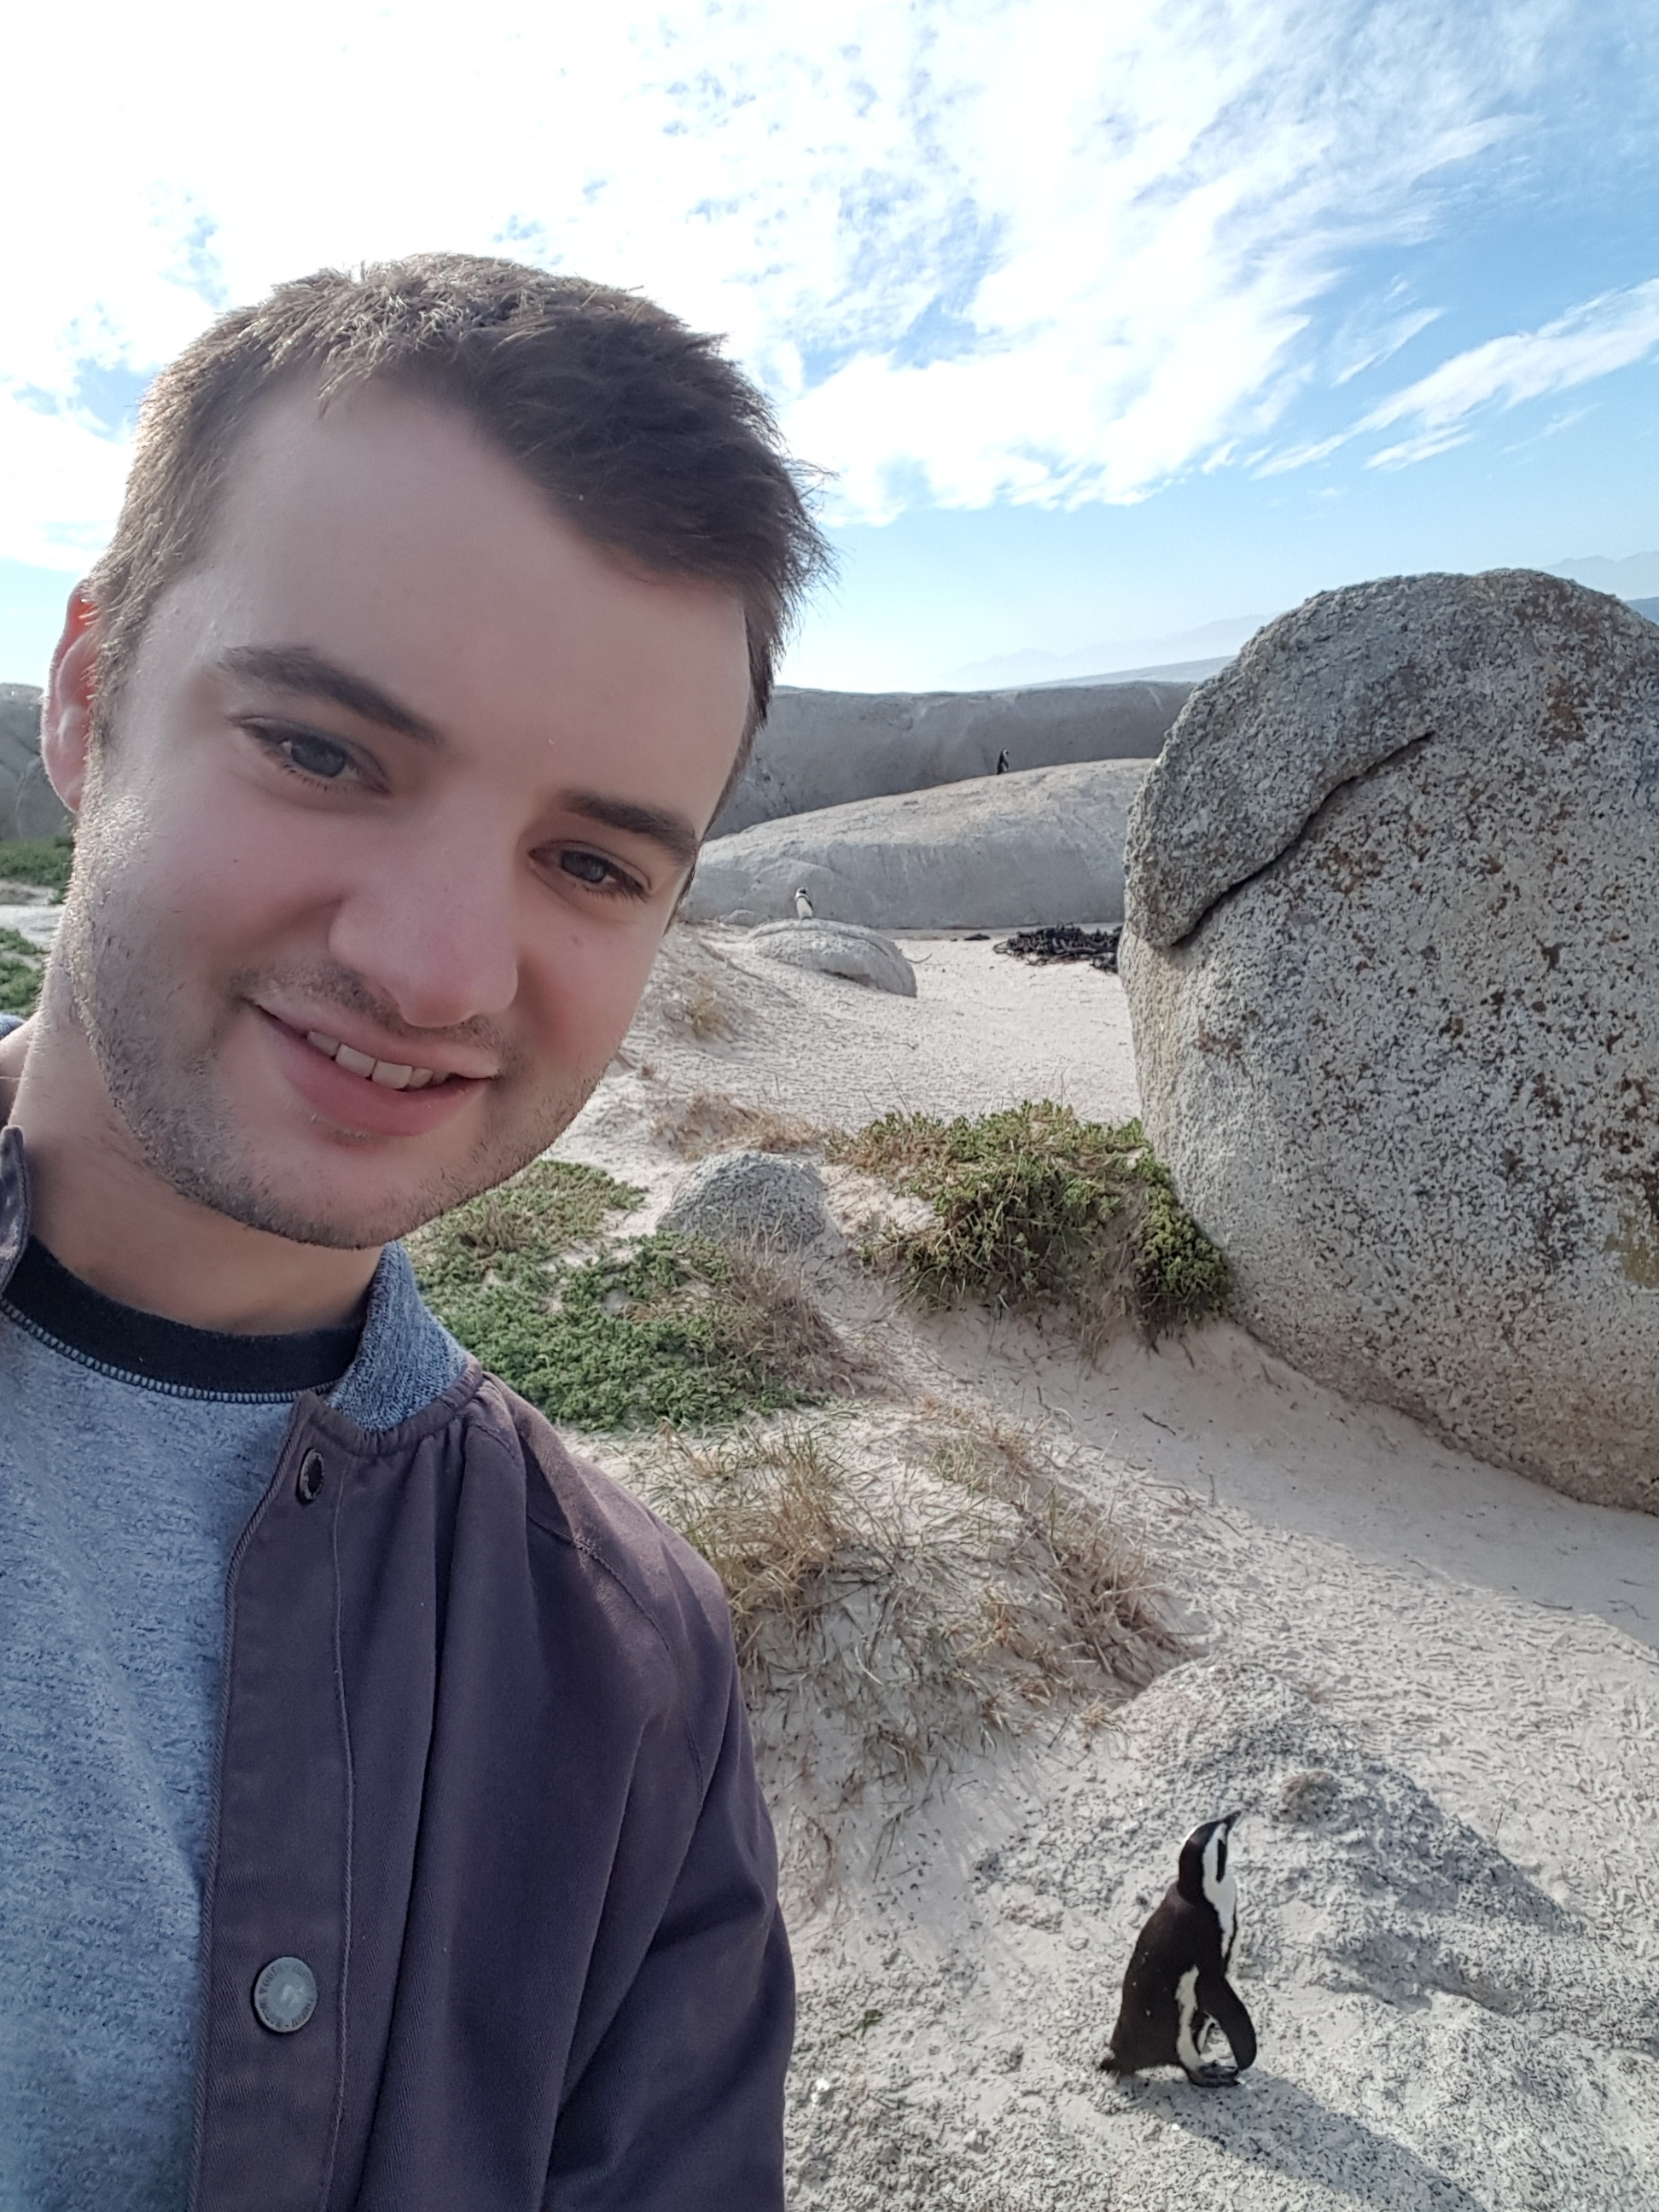
\includegraphics[width=\textwidth]{IMAGES/MikePenguin}
	 };            
         \node[anchor = north east, text width = 0.4\linewidth, xshift=-4cm, yshift=-0.25cm] at (current page.north east) {
   	    \centering
            Otto lab\\
   	    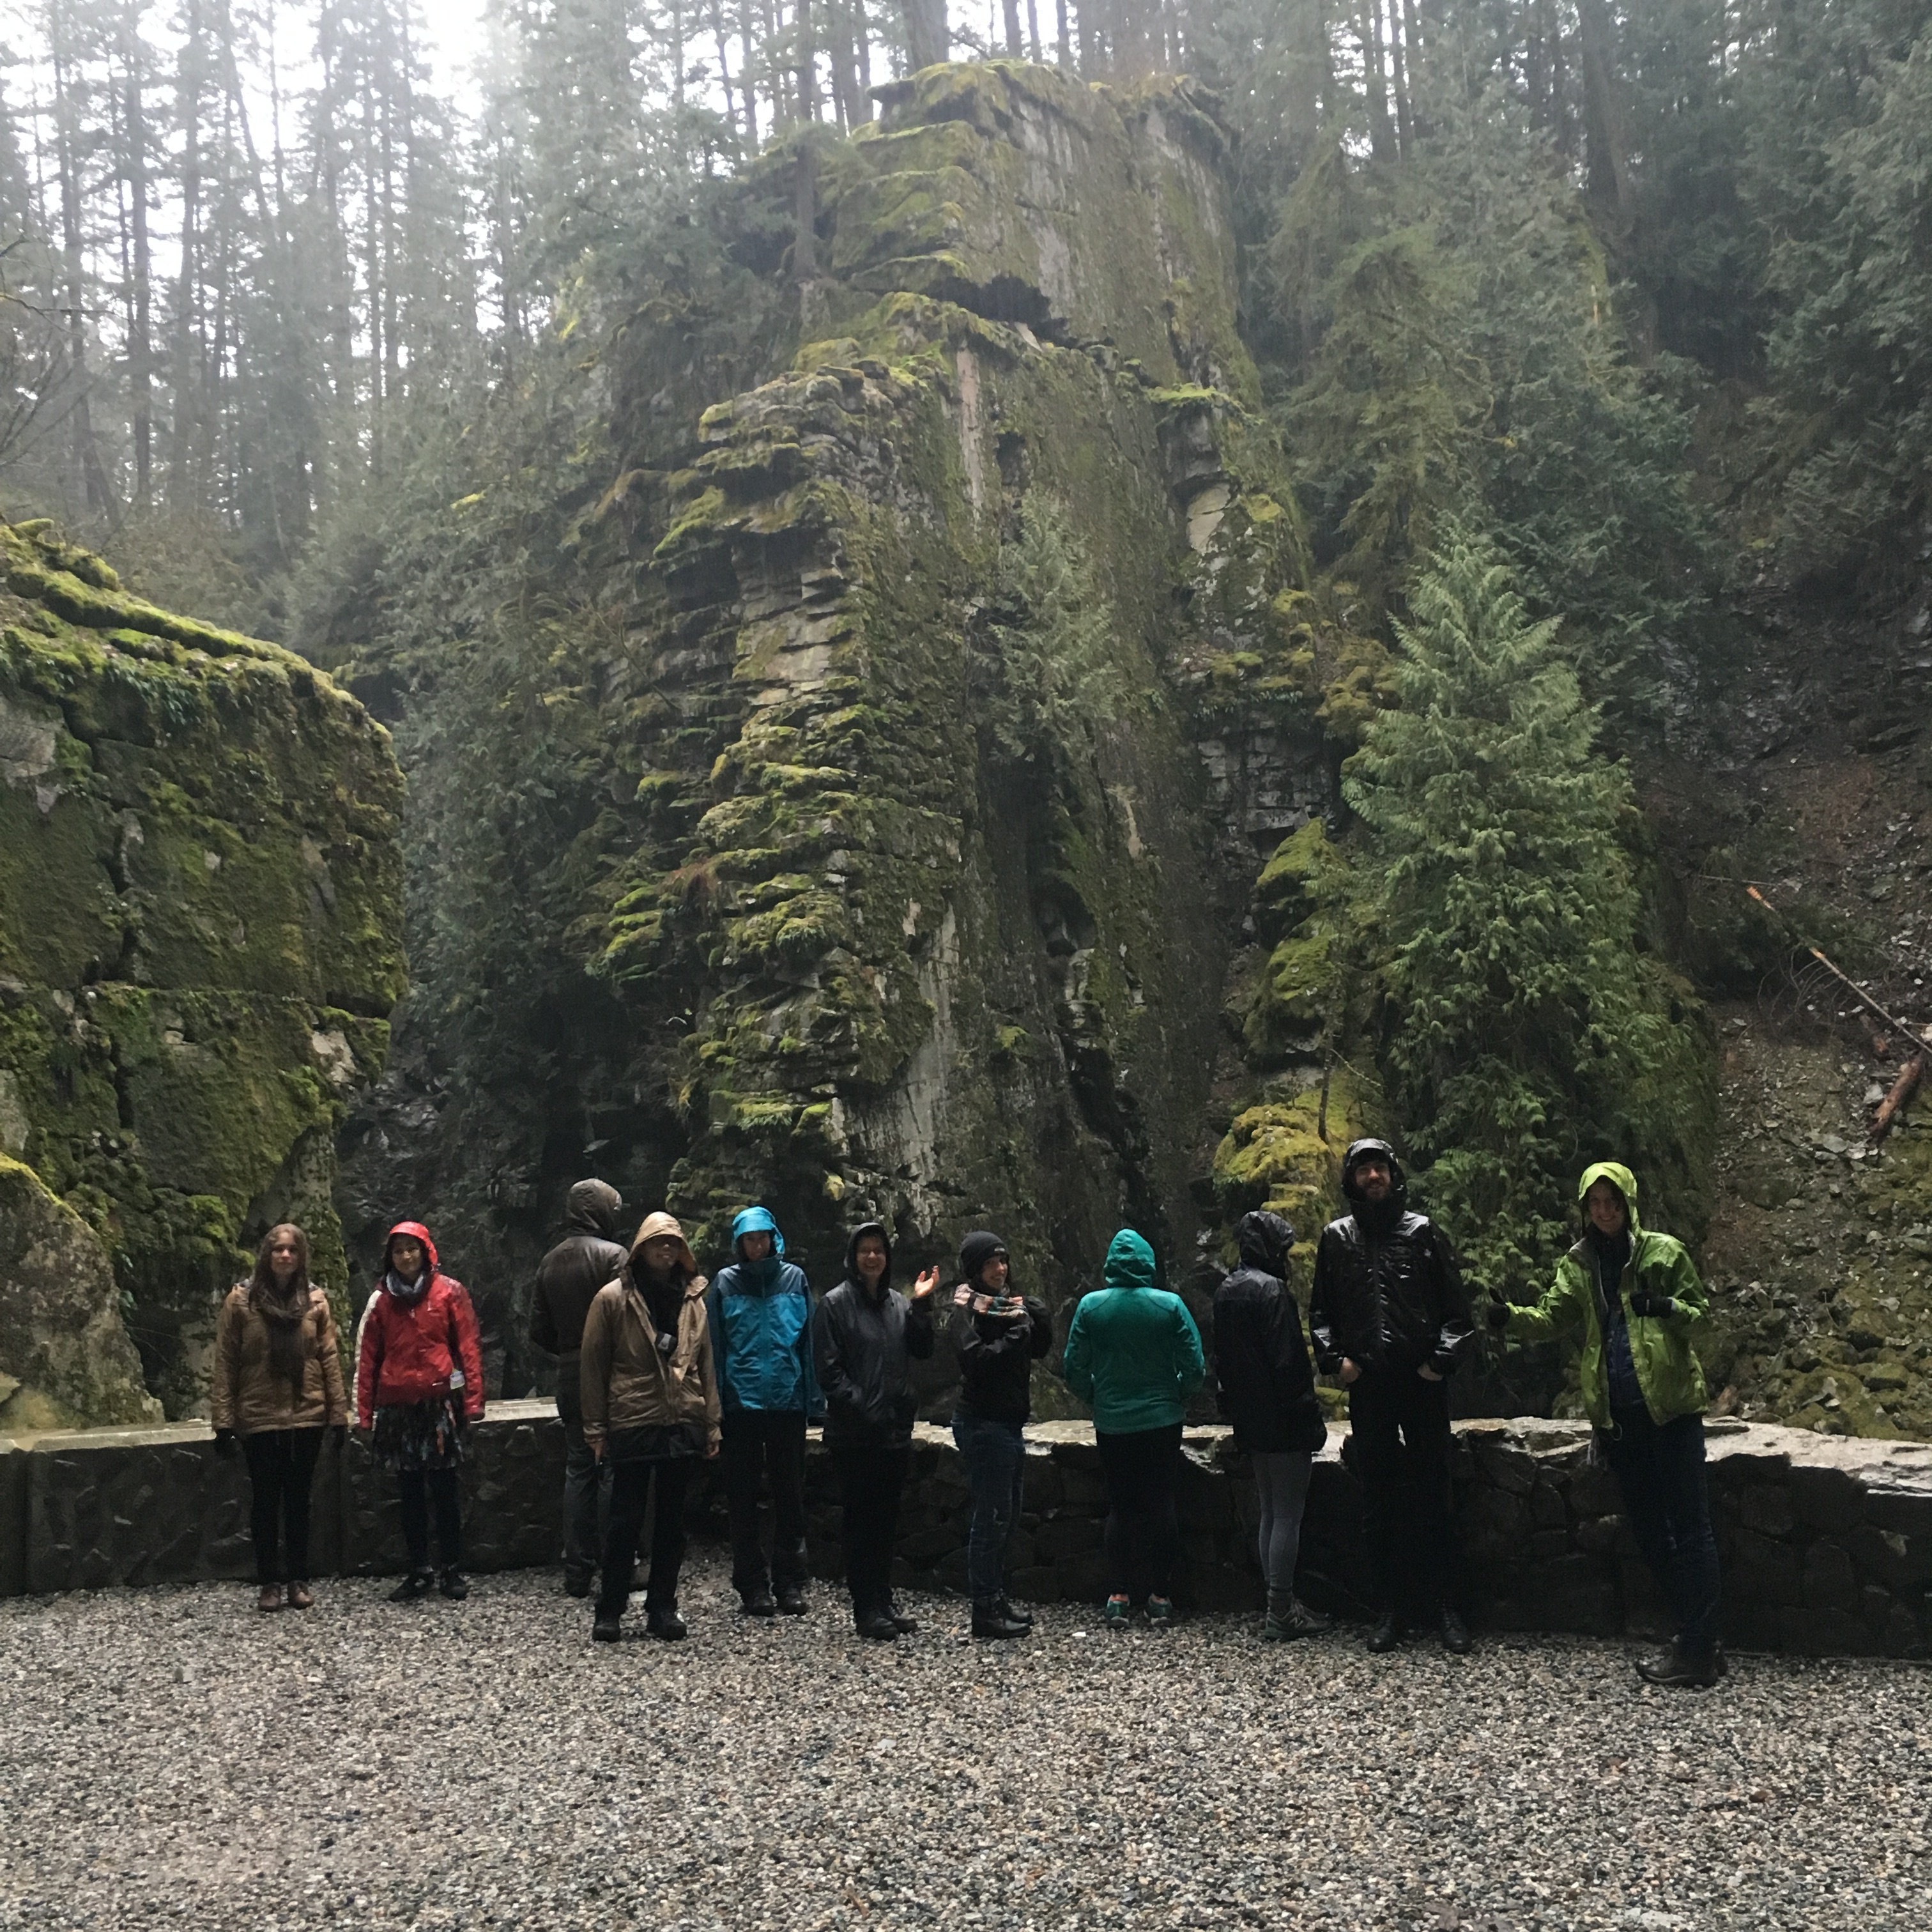
\includegraphics[width=\textwidth]{IMAGES/OttoLab}
	 };     
         \node[anchor = east, text width = 0.4\linewidth, yshift=-0.75cm] at (current page.east) {
   	    \centering
            Sally Otto\\
   	    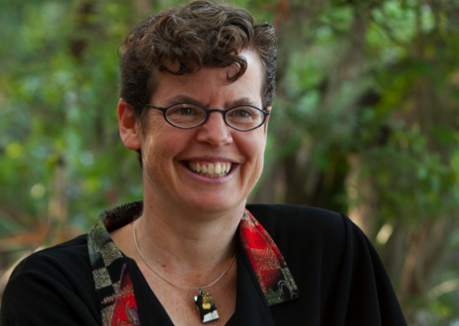
\includegraphics[width=\textwidth]{IMAGES/Sally}
	 };     
         \node[anchor = south west, yshift=0.7cm] at (current page.south west) {
   	    
\includegraphics[width=0.5\textwidth]{IMAGES/BRC}
	 };     
         \node[anchor = south, xshift=1cm] at (current page.south) {
	    
\includegraphics[width=0.15\textwidth]{IMAGES/UBC}
	 };     
         \node[anchor = south east, yshift=0.5cm] at (current page.south east) {	    			   		
            
\includegraphics[width=0.3\textwidth]{IMAGES/NSERC}
	 };   	   
   \end{tikzpicture}
\end{frame}
%%%%%%%%%%%%%%%%%%%%%%%%%%%%%%%%%%%%%%%%%%%%%%%%%

\end{document}